 % !TEX program = xelatex

\documentclass[titlepage,UTF8,linespread=1.5]{ctexart}
\ctexset {
    % 段落标题独立成行
    paragraph/runin = false,
    subparagraph/runin = false
}

% 开启图片功能,定义图片目录
\usepackage{graphicx}\graphicspath{{image/}}
% 强制定位
\usepackage{float}
% 首段开启缩进
\usepackage{indentfirst}
% 页边距
\usepackage[margin=1.25in]{geometry}
% 段落边框
\usepackage{mdframed}
% 长表格
\usepackage{longtable}
% 超链接,放在最后避免冲突
\usepackage[unicode,hidelinks]{hyperref}

% 页眉页脚
\pagestyle{plain}

% 设定图片独占一页偏移量
\makeatletter
\setlength{\@fptop}{0pt}
\makeatother

% 设定默认字体
\setmainfont[BoldFont={Times New Roman Bold}, ItalicFont={Times New Roman Italic}]{Times New Roman}
\setsansfont[BoldFont={Times New Roman Bold}, ItalicFont={Times New Roman Italic}]{Times New Roman}
% \setmonofont[BoldFont={Times New Roman Bold}, ItalicFont={Times New Roman Italic}]{Times New Roman}

% 加载自定义字体
\setCJKfamilyfont{xingkai}{行楷-简}
\newcommand{\xingkai}{\CJKfamily{xingkai}}

% 重定义封面
\renewcommand{\maketitle}{\begin{titlepage}
\begin{center}
{\xingkai \zihao{-0}上海电力学院}
\\[36pt]
{\fangsong \zihao{-0}本科毕业设计(论文)}
\\[36pt]

\includegraphics[height=45mm, width=45mm]{logo-shiep.png}
\\[36pt]
{\zihao{4}
\renewcommand\arraystretch{1.2}
\begin{tabular}{rc}
    \makebox[4em][s]{题\hspace{\fill}目}:& \underline{\makebox[15em]{基于Spring MVC}} \\
                                         & \underline{\makebox[15em]{课程资源网站设计与实现}} \\
    \makebox[4em][s]{院\hspace{\fill}系}:& \underline{\makebox[15em]{计算机科学与技术学院}} \\
    \makebox[4em][s]{专业年级}:          & \underline{\makebox[15em]{网络工程2014级}} \\
    \makebox[4em][s]{学生姓名}:          & \makebox[15em][s]{\underline{\makebox[5em]{潘成}}\hspace{\fill}
                                          学号:\underline{\makebox[6em]{\phantom{|}20142520\phantom{|}}}} \\ 
    \makebox[4em][s]{指导教师}:          & \underline{\makebox[15em]{周平}} \\
    & \\
    & \makebox[15em][r]{\today}
\end{tabular}
}
\end{center}
\end{titlepage}}

% 正文开始
\begin{document}
\maketitle

{\renewcommand\abstractname{\heiti\zihao{3}{基于Spring MVC课程资源网站设计与实现}\\[16pt]\zihao{4}{摘要}}
    \begin{abstract}\par
        随着计算机、互联网、网络技术的发展和第四代移动通讯技术的普及,在线教育已经逐渐成为一个热门话题,并日渐融入到人们生活中去,
        建设在线教育平台已成为各大高校现代化建设的一项重要的组成部分。教育的本质是信息传递的行为,相比于传统的教学方式,在线教育
        平台能通过多媒体技术整合丰富的教育资源,借助互联网技术突破地理位置的限制,减小教育资源的差异化,提高教育质量。\par
        本文依照软件工程的开发流程详细论述了一个基于Spring MVC课程资源网站设计与实现的过程,该系统参考其他高校在线课程资源中心,
        以及现有成功商业在线教育平台,如慕课网等网站,从我校实际出发,制定系统需求分析。该系统分为权限模块、课程资源模块、在线测试
        模块、论坛模块、文件模块组成,界面友好,配置灵活,可呈现丰富的在线教育资源类型。\par
        本系统采用采用软件行业较为前沿的技术,整体使用B/S架构,同时基于前后端分离的方案设计。后端使用Kotlin\cite{kotlin}语言
        开发,采用Spring Cloud\cite{spring-cloud}微服务架构,基于nginx搭建网关和文件服务器,使用MySQL和Redis作为持久化
        存储工具,Gradle\cite{gradle}作为项目管理工具;前端使用JavaScript语言开发,采用Vue\cite{vue}框架、Element-UI组
        件,使用Webpack\cite{webpack}作为项目管理工具。统一使用Git作为源码版本控制工具,部署在阿里云服务器上。\par
        \vspace{1em}
        \noindent\textbf{\heiti\zihao{-4}关键词:} 在线教育,课程资源网站,Spring,Kotlin,Vue
    \end{abstract}
}

{\renewcommand\abstractname{\heiti\zihao{3}{Design and Implementation of Curriculum Resources Website
            Based on Spring MVC}\\[16pt]\zihao{4}{Abstract}}
    \begin{abstract}\par
        With the development of computers, Internet, and network technologies, and the popularity of 4G, online
        education has gradually become a hot topic and has gradually become integrated into people’s lives.
        Building an online education platform has become an important part of the modernization of universities.
        The essence of education is the behavior of information transfer. Compared with traditional teaching methods,
        online education can integrate rich educational resources through multimedia technology, and use Internet
        technology to break through the limitation of geographical location, reduce the differentiation of
        educational resources, and improve the quality of education.\par
        This article discusses the process of designing and implementing a curriculum resources website based on
        Spring MVC according to the development process of software engineering in detail. The system refers to
        the online resource centers of other colleges and universities, as well as the existing successful commercial
        online education platforms, such as mooc etc. and proceed from reality of our school, to analysis system
        requirements. The system composes of permission module, curriculum resource module, work and examination
        module, forum module and file module. The interface is friendly, and the configuration is flexible. It can
        present a rich type of online education resources.\par
        This system adopts the more advanced technology of the software industry, uses the B/S architecture as a whole,
        and is designed based on the separation of the front and back ends. The backend is write in Kotlin\cite{kotlin}
        language, using the Spring Cloud\cite{spring-cloud} microservice architecture, building gateways and file
        servers based on nginx, using MySQL and Redis as database, Gradle\cite{gradle} as a project management tool,
        front end wirte in JavaScript language, using Vue\cite{vue} framework, Element-UI components, use Webpack
        \cite{webpack}as a project management tool. Uniformly use Git as source version control tool and deploy on
        Alibaba Cloud server。\par
        \vspace{1em}
        \noindent\textbf{\heiti\zihao{-4}Keywords:} Online Education, Curriculum Resources Website, Spring, Kotlin, Vue
    \end{abstract}
}

\tableofcontents
\clearpage

\section{绪论}
\subsection{目的}
随着计算机、互联网、网络技术的发展和第四代移动通讯技术的普及,在线教育已经逐渐成为一个热门话题,并日渐融入到人们生活中去,
人们对教育的要求也越来越高,探索新的教育方式是刻不容缓的需求。教育的本质是信息传递的行为,相比于传统的教学方式,在线教育
平台能通过多媒体技术整合丰富的教育资源,借助互联网技术突破地理位置的限制,减小教育资源的差异化,提高教育质量。本项目致力于
借助现有的软件行业前沿技术,从我校实际需求出发,探索建设一个在线课程资源网站,以满足教育现代化建设需求。\par
本篇论文详细论述了课程资源网站项目设计与实现的过程,从需求分析到概要设计到数据库设计、详细设计以及最后的测试报告。\par
\subsection{背景}
国务院总理李克强在2017年政府工作报告\cite{2017政府工作报告}中提及“在线教育”,指出“扩大数字家庭、在线教育等信息消费”。在此之前,“在线教育”
已经多次在往届两会中被提及,而这是首次被正式写入政府工作报告。\par
据中国互联网络信息中心发布的第40次《中国互联网络发展状况统计报告》\cite{第40次中国互联网络发展状况统计报告}显示,截至2017年6月,
中国在线教育用户规模已达1.44亿人次,相比于2016年底增加662万人,半年增长4.8\%。其中,手机在线教育用户规模为1.20亿人次,相比于2016年底增长
2192万人,增长率为22.4\%。报告显示,各类精准教学、网络课程正日渐成为课堂学习、正规教育的有益补充,使教育资源得到优化配置、教育不受时间空间
限制,使教育的方法方式变得越来越多元化。\par
\subsection{意义}
本课题主要研究构建一个配置灵活、自主可控的课程资源管理系统。虽然目前市场上已有大量的类似系统,但灵活方面略显不足,面对各类具体需求时还需定制
和二次开发,并且 在后续的修改和维护中还要依赖开发商本身,始终处于被动的局势。 因此,自主设计一个灵活、可控的课程资源管理系统是十分有意义的。\par
\subsection{国内外发展状况}
MOOC(Massive Open Online Course)即“大规模在线开放课程”,具有大规模和开放性等特点,已日渐成为国内外研究的热点。\par
在MOOC的流行起来之前,我国高等教育已经有很多网络课程资源建设的探索。2000年教育部高教司面向高校方式“新世纪网络课程建设工程”,随后于2003年
教育部又启动了“国家精品课程建设工程”,截至2010年共评选出3800多门国家精品课程,上万省级、校级的精品课程。2010年起,以耶鲁大学为代表的知名
高校的视频公开课逐渐在网络上流行,国内一些互联网企业,如网易也创建了网易公开课项目,掀起了网络公开课的学习浪潮。2011年,教育部启动了“国家精
品开放课程建设工程”,进一步在精品课程的基础上开放共享。\par
因此可以说在MOOC流行之前,国内对于在线学习的建设已有一定的基础。2012年MOOC风暴掀起之后,国内诸多高校纷纷跟进。北京大学、清华大学、上海交大、
复旦大学等知名高校纷纷加入Courser和edX等MOOC平台。2013年,清华基于open-edX开源项目,研发了自主MOOC平台“学堂在线”,2014年上海交大自主
研发的“好大学在线”平台也正式发布,并与西南片高校跨校合作,学分互认。同一年,深圳大学带头组建UOOC联盟,以联高校盟的形式推动MOOC建设,并与企
业合作构建MOOC平台。高校之外,爱课程网和网易云课堂合作推出的“中国大学MOOC”,2012年组建的“上海课程中心”等,也汇聚了大量优质的在线课程资源。\par
\subsection{系统主要研究内容}
\begin{itemize}
    \item 如何实现一套灵活的权限控制系统。
    \item 如何实现一个支持丰富种类展示与编辑的在线课程资源系统。
    \item 如何实现图片、视频等文件的上传、存储、下载与在线展示。
    \item 如何实现在线测试系统。
    \item 如何实现一个在线交流论坛。
    \item 对Spring Cloud微服务架构的探索。
\end{itemize}
\clearpage

\section{需求分析}
\subsection{引言}
\subsubsection{目的}
编写本课程管理系统需求分析说明书的目的是:明确本系统相关使用人员对本系统的功能、行为和性能等方面的要求,准确定位需求;研究现有的类似系统,
总结设计系统的总体方案;对设计方案进行技术、经济、社会等方面的可行性分析,得出是否本系统是否值得开发的结论。\par
\subsubsection{背景}
在国家十三五规划的指导下,在大规模在线开放课程热潮的推动下,为推动国家“互联网+教育”战略发展,推进数字教育资源普遍开放共享,推动我校现代化
教育建设,现在我院迫切需要研发一个自主灵活的在线课程资源系统。\par
在此背景下,本平台的开发需求应运而生。\par
\subsubsection{用户特点}
系统面向系统管理员、高校教师、在校学生以及其他互联网网民。其中高校师生及大部分网民具备基本的计算机操作能力,本系统应力求做到逻辑简单,界面
友好,符合常规思考逻辑,同时提供强大自制配置能力和干净、易于扩展的二次开发接口和文档,又不失灵活性。\par

\subsection{任务描述}
\subsubsection{功能要求}
\paragraph{权限控制}
可在运行期动态定义用户-角色-权限及其绑定关系。\par
可扩展,允许对资源本身进行细粒度的权限控制。\par

\paragraph{课程资源}
支持多样化的课程资源上传、管理、浏览,包括但不限于演示文档、视频、文字等形式。\par
\paragraph{在线测试}
支持自定义题库,有题目生成试卷,可以在线浏览试卷测试题和答案。\par
\paragraph{在线论坛}
支持板块、发帖、回帖等基本功能,被授权者可以关闭、删除帖子。\par

\subsubsection{性能要求}
\paragraph{时间特性要求}
\begin{enumerate}
    \item 大量展示数据应按需加载、分页加载,提高载入速度。
    \item 系统页面响应时间在网络连接正常的情况下应不超过2秒。
    \item 数据转换与交互时间应不超过2秒。
    \item 系统应减少与数据库的连接次数。
\end{enumerate}

\paragraph{输入输出要求}
本系统后台接口统一采用RESTful风格设计,易于交互,方面后期自主开发扩展其他平台应用,如安卓移动端、系统集成等。\par
同时可以针对接口实现细粒度权限控制,满足不同场景的具体使用需求。\par

\paragraph{灵活性要求}
\begin{enumerate}
    \item 系统兼容目前市场上各大主流浏览器。
    \item 部分数据检索条件应支持模糊查询。
    \item 系统模块化部署,对于部分服务器故障,系统具备一定的容灾能力。
\end{enumerate}

\paragraph{故障处理要求}
服务器使用阿里云服务器,每周定期对系统进行快照备份,可以对系统进行快速的恢复,预防硬盘损毁等灾难性故障带来的系统长期离线状态。\par
数据库数据定期导出备份,避免数据损坏。\par
分布式部署,多实例、多机器集群部署,提高系统的容灾能力,避免单机物理故障造成系统的整体瘫痪。\par

\subsection{可行性分析}
\subsubsection{技术可行性}
系统采用前后端分离设计方案,通过RESTful接口进行数据交互。整个工程项目使 用Git版本控制工具管理。\par
\paragraph{前端技术选型}
\begin{itemize}
    \item 开发语言:Html、CSS、JavaScript
    \item 开发框架:Vue、Element-UI、Vue Router、Vuex、axios
    \item 项目管理:Webpack3、Babel
    \item 开发环境:Deepin Linux 15.5、OSX 10.13、Node 8.9
    \item 开发工具:VSCode、WebStorm
\end{itemize}\par
前端框架选择了Vue技术栈。Vue框架作为目前三大前端框架(其它两者为Angular、React)之一,功能丰富,同时简单易学。Vue一大特色是主张渐进式的
学习,有十分平缓的学习曲线,同时中文文档齐全,生态良好,社区活跃,并经受住市场的考验,国内著名的B站前端即使用Vue框架实现,是一个稳定、可
靠的框架。\par
Webpack3的Babel转码插件保证了前端页面的兼容性,可兼容当前市面上除IE8以下的所有主流浏览器。\par

\paragraph{后端技术选型}
\begin{itemize}
    \item 开发语言:Kotlin
    \item 开发框架:Spring Boot、Spring Cloud、Spring Data、Spring MVC
    \item 数据存储:MySQL、Redis
    \item 项目管理:Gradle
    \item 开发环境:Deepin Linux 15.5、OSX 10.13、OpenJDK 1.8
    \item 开发工具:Intellij IDEA
\end{itemize}\par
后端框架选择了Spring技术栈。\par
Koltin是一门多平台、多范式的新语言,它由JetBrains\cite{jetbrains}——最优秀的商业IDE公司团队设计,吸收了众多编程语言的优秀特性。Koltin
定位工程实践,它的JVM平台部分完全兼容Java语言及现有的Java库,在此基础上,Koltin将面向对象中常用的设计模式内置到语法特性中,支持函数式编程、
协程、具名参数、内联函数等众多实用特性。Kotlin总结了Java语言诞生以来20余年的工程经验,大大丰富了语言特性,是对Java语言一个强大的补充。
Google Android和Spring 5已经官方支持Kotlin。\par
Spring框架在Java EE开发中占据绝对的主导地位,Spring的核心是IoC和AOP。IoC是对OOP的完美演绎,AOP是对OOP的正交互补。Spring Cloud是一套
功能完善的分布式微服务应用解决方案,保证了应用极强的扩展能力。Spring本身既提供一站式的解决方案,同时各模块间的耦合松散,兼容各大主流框架,可
以完全自主灵活地选择技术组合。本应用后台除权限模块外,全部使用Spring框架,既保证了权限系统的灵活性,又保证了整个后台系统的稳定、可靠性。\par
Gradle是新一代项目管理工具,兼容Maven、Ant的一切特性,拥有庞大的插件库,并直接支持Groovy脚本扩展功能,是一个强大、灵活的项目管理工具。\par
MySQL是一个轻巧、性能良好、易用的开源数据库,有广泛的使用群体和技术解决方案,能满足高并发、可集群的需求;Redis是一个基于内存的NoSQL,可作为
分布式缓存使用。\par

\paragraph{测试部署平台}
\begin{itemize}
    \item 硬件平台:阿里云主机3台,单核CPU、2G内存
    \item 操作系统:Ubuntu Server 16.04 x64、Linux Kernel 4.4
    \item 运行环境:Open JDK 1.8、Node 8.9、MySQL 5.7、Embedded Tomcat(Spring Boot内嵌)、Redis 3.0、Nginx 1.10
\end{itemize}\par
阿里云通过虚拟化技术提供云主机,可根据实际性能需求弹性购买硬件资源。阿里云经过多年电商平台、各大企业的考验,证明了其是一个技术成熟、稳定可
靠的云服务器平台。\par
Ubuntu Server 16.04是使用广泛的服务器系统,它基于Linux内核发开,稳定、高效。\par
Nginx用于部署前端应用,搭建文件服务器,以及作为网关为后端服务反向代理和负载均衡;后端服务直接由Spring Boot内嵌Tomcat容器启动。\par

\subsubsection{经济可行性}
本系统使用的技术方案和开发工具多为开源作品,完全遵守版权规定,可以免费使 用。其中Intellij IDEA和WebStorm为JetBrains公司发行的商业软件,
但该公司为高校师生提供免费教育许可证,可以免费用于非商业目的。\par
根据对并发性能的需求,本系统可以做到弹性部署,在并发需求不高时,可单机部署;当某些功能并发量较大时,可单独对该模块分配较多资源或集群部署,做
到资源最大化的利用,降低经济成本。\par
同时本系统设计灵活,提供强大的配置功能,可以满足多种具体使用场景,降低了定制开发的经济成本。\par
\subsubsection{社会可行性}
本系统的设计、开发、应用完全遵守法律法规,对在线教育事业有积极的促进作用,具备社会可行性。\par

% \subsection{数据流图}
% \subsubsection{顶层图}
% % todo
% \subsubsection{0层图}
% % todo
% \subsubsection{1层图}
% % todo
% \clearpage

\section{概要设计}
\subsection{总体设计}
从网站界面上来看,系统整体上分为前端展示界面和后台管理界面两大部分,以及一个登录界面。\par
从模块功能上看,系统模块结构如图\ref{fig:struct-module}所示。\par
\subsubsection{系统模块结构图}
\begin{figure}[H]
    \centering
    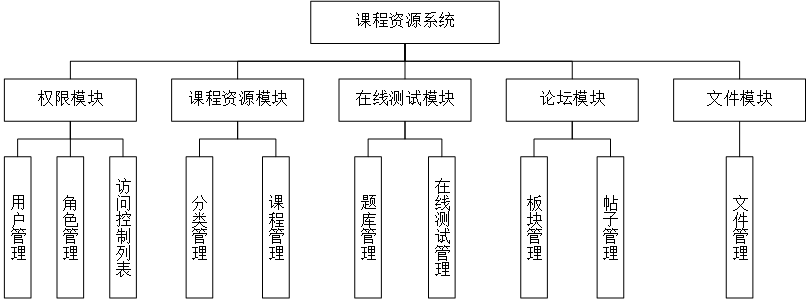
\includegraphics[width=150mm]{struct-module.png}
    \caption{系统模块结构图}
    \label{fig:struct-module}
\end{figure}
\subsection{系统模块功能}
\begin{figure}[H]
    \centering
    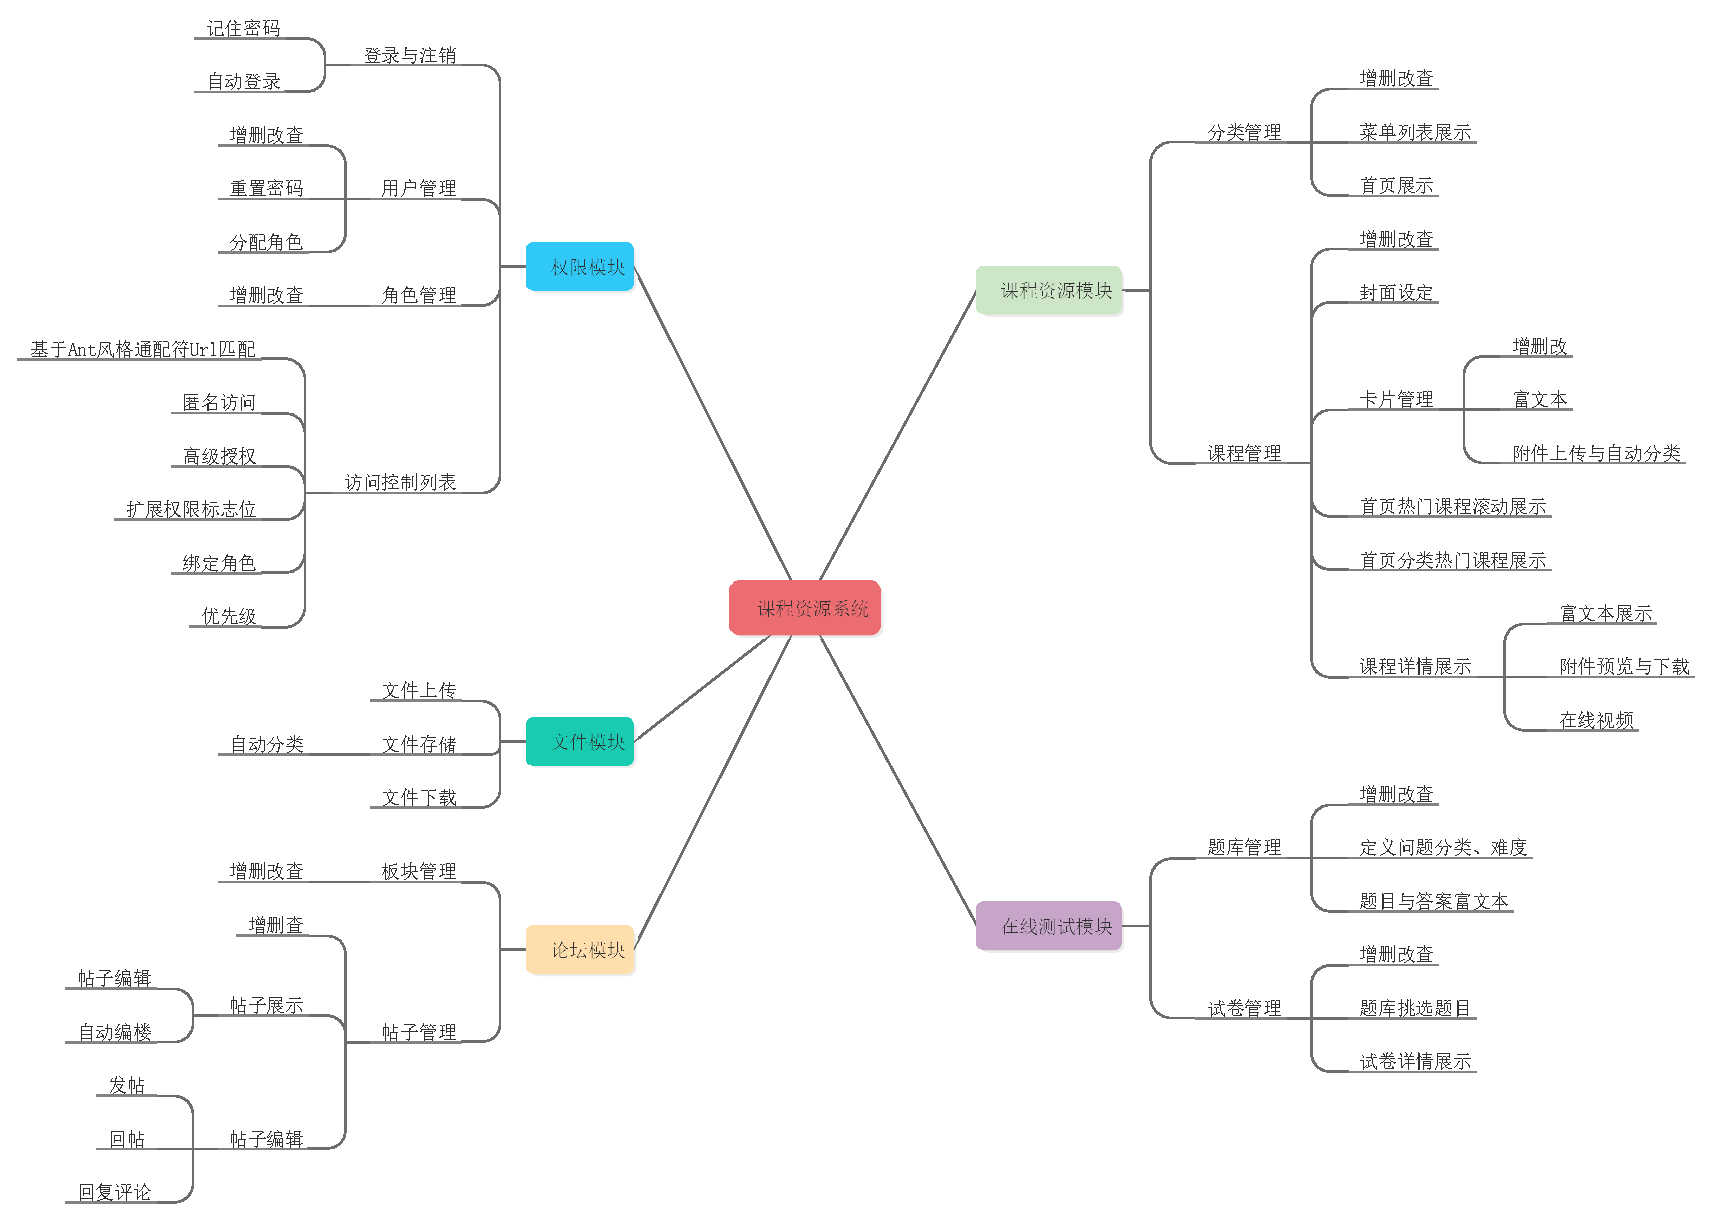
\includegraphics[width=150mm]{mind-overall.eps}
    \caption{系统功能设计思维导图}
    \label{fig:mind-overall}
\end{figure}

\subsubsection{权限模块}
\paragraph{登录与注销}
允许用户根据登录名和密码自助登录,提供记住密码、自动登录功能。登录后允许用户自动注销,同时清除自动登录状态。\par
\paragraph{用户管理}
在后台管理界面,向系统管理员或被授权者提供用户管理功能,可以增加、修改、删除用户,允许根据用户名、登录名模糊检索用户;可以强制重置用户密码;
可以动态的为用户分配角色,以授予不同的权限。\par
\paragraph{角色管理}
在后台管理界面,向系统管理员或被授权者提供角色管理功能,在后台管理界面,可以增加、修改、删除角色,允许根据编码、名称模糊检索角色。\par
\paragraph{访问控制列表}
在后台管理界面,向系统管理员或被授权者提供基于URL级别的访问控制列表管理功能,允许增加、修改、删除规则,允许根据用户名、URL模糊检索,根据是
否允许匿名访问精确检索。在定义规则时,URL支持Ant风格的通配符;提供匿名访问和高级授权标志位,以及用于后续自定义扩展的标志位列表;允许将规则
应用到角色上;允许设定规则优先级,优先级数值越小,优先级越高,在匹配时,第一条匹配成功的规则生效。\par

\subsubsection{文件模块}
\paragraph{文件上传}
允许向服务器上传各种类型的文件,包括但不限于图片、视频、音乐、文档等类型,可以根据文件扩展名对常见类型文件自动分类。考虑到服务器压力,允许上传
的最大单个文件为100MB。服务器自动将文件按一定规则存储到磁盘中,并向请求方范围一个URL,用于下载该文件。\par
\paragraph{文件下载}
根据客户端发送请求的URL到服务器磁盘指定位置查找文件,若查找到,向客户端传输文件;若查找不到,返回错误提示信息。\par

\subsubsection{课程资源模块}
\paragraph{分类管理}
在后台管理界面,允许管理员或被授权者管理课程分类,可以增加、修改、删除分类,可以根据名称模糊检索分类。\par
在首页展示界面上,会展示所有版块,在前端展示菜单栏上,会显示所有的分类,点击后显示该分类下所有的课程。\par
\paragraph{课程管理}
课程需要指定分类、教师,课程可以设定封面,课程内容由卡片组成,每个卡片支持定义标题,包含一个Markdown富文本编辑器,支持上传附件,附件自动识别
Excel、Word、PPT、压缩包、PDF、视频格式,PDF支持在线预览,视频支持在线观看。\par
在后台管理界面,允许管理员或被授权者管理课程,可以增加、修改、删除课程,可以根据分类、课程名、教师检索课程;允许课程动态绑定、编辑、删除卡片。\par
首页展示界面上,滚动展示最新课程,显示每个类别的最新课程。在前端课程搜索界面上,可以根据分类、课程名、教师搜索课程。在课程详情界面,展示课程介绍、
图片、所有卡片内容,PDF支持在线预览,视频支持在线观看,其他类型附件支持下载。\par

\subsubsection{在线测试模块}
\paragraph{题库管理}
题目由问题和答案组成,问题和答案内容均由Markdown富文本展示,可以展示丰富的内容形式。\par
在后台管理界面,允许管理员或被授权者管理题库,可以增加、修改、删除题目,可以根据课程、教师、类型检索题目。\par

\paragraph{试卷管理}
试卷需要指定课程,试卷由题目组成。\par
在后台管理界面,允许管理员或被授权者管理试卷,可以增加、修改、删除试卷,可以根据课程、名称模糊检索试卷;可以从题库中挑选题目组成试卷。\par
在前端在线测试搜索界面,允许根据课程、名称模糊检索试卷,点击“开始测试”按钮进入该测试对应的详情页。试卷详情页首部展示试卷标题、课程、简介等信息,
以及所有的题目信息,默认答案隐藏,可以点击查看题目答案。\par

\subsubsection{论坛模块}
\paragraph{版块管理}
在后台管理界面,允许管理员或被授权者管理论坛版块,可以增加、修改、删除版块,可以根据名称模糊检索版块。\par
在前端交流论坛界面,展示所有版块,点击每个版块展示该版块内的帖子。\par
\paragraph{帖子管理}
帖子由标题、发言及一系列的发言组成。\par
在后台管理界面,允许管理员或被授权者管理帖子,可以删除帖子,可以根据版块、标题、关键字检索帖子。\par
在前端交流论坛界面,允许根据标题、关键字模糊检索帖子,根据版块查询帖子,帖子列表上展示标题、最新回复时间、发言总量等信息,点击帖子标题,进入帖子
详情。在帖子详情页,展示帖子详情及每条发言信息,发言自动编号楼层,可以回复楼主或任一条发言,新发言会标注所回复的发言。\par

\subsection{用户界面设计}
系统整体上分为前端展示界面和后台管理界面两大部分,以及一个登录界面。前端界面主要面向网站一般访客、学生等群体,后台管理界面主要面向管理员、课程
信息编辑者、教师等群体。管理员以及被授权的用户在登录后在前端展示与后台管理界面之间切换。\par
\subsubsection{登录界面}
\begin{figure}[H]
    \centering
    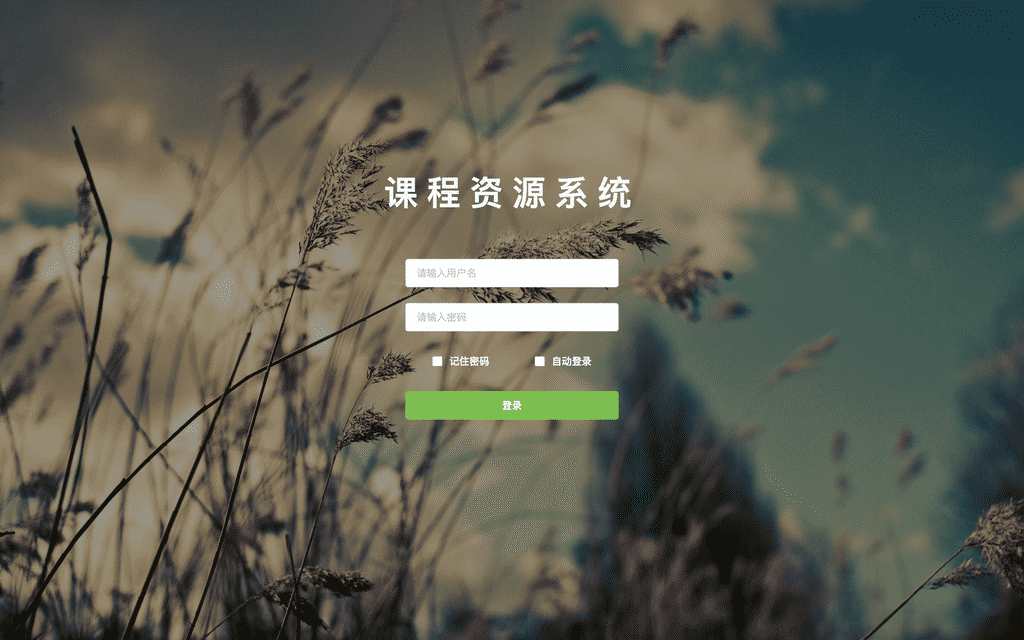
\includegraphics[width=140mm]{view-login.png}
    \caption{登录页}
    \label{fig:view-login}
\end{figure}
\subsubsection{前端展示界面}
\begin{figure}[H]
    \centering
    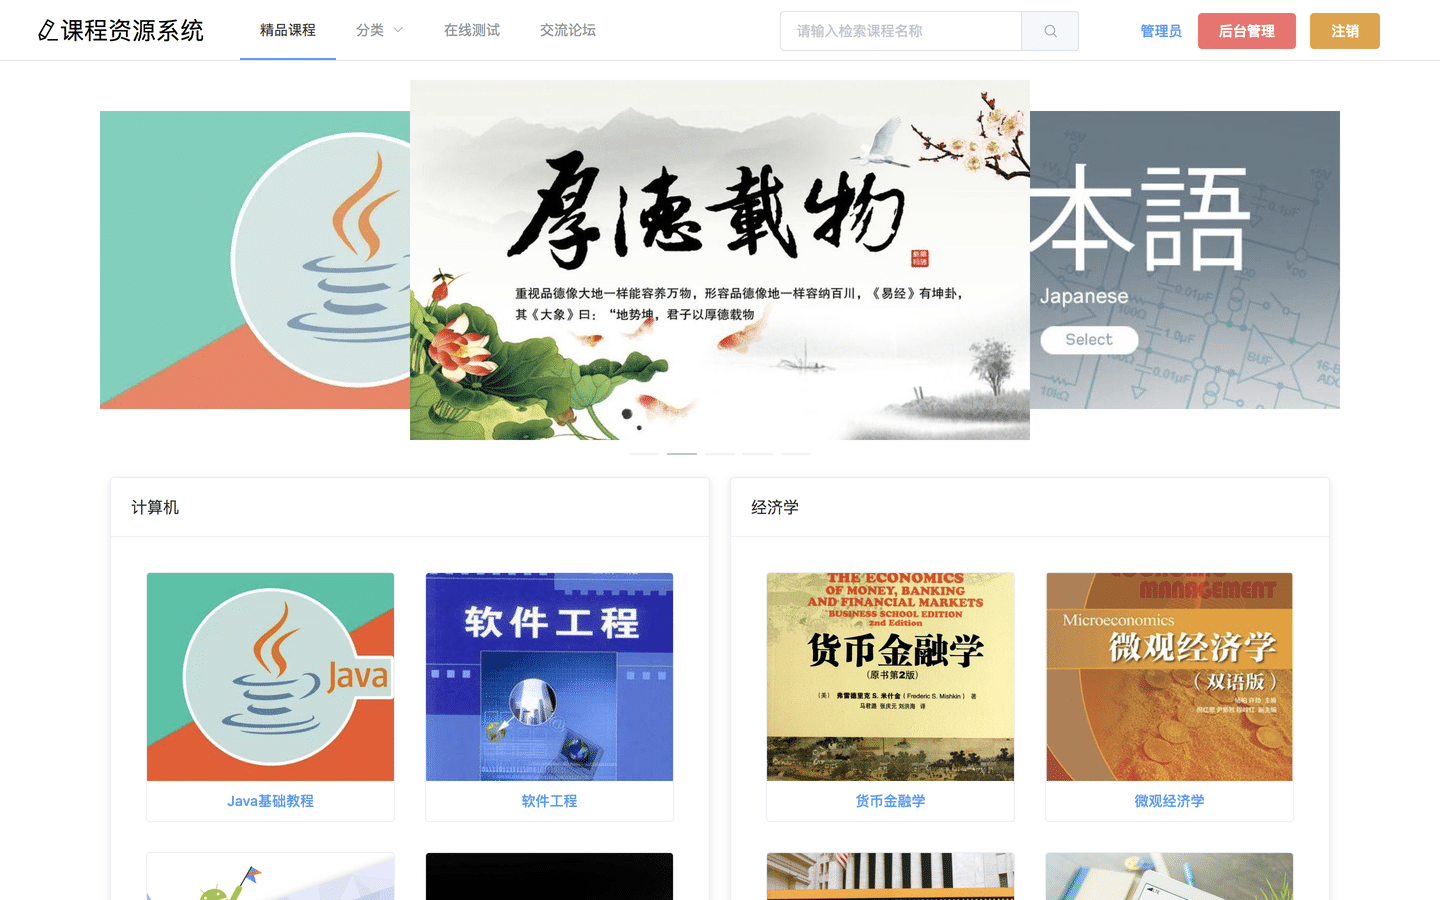
\includegraphics[width=140mm]{view-home.png}
    \caption{主页}
    \label{fig:view-home}
\end{figure}
\begin{figure}[H]
    \centering
    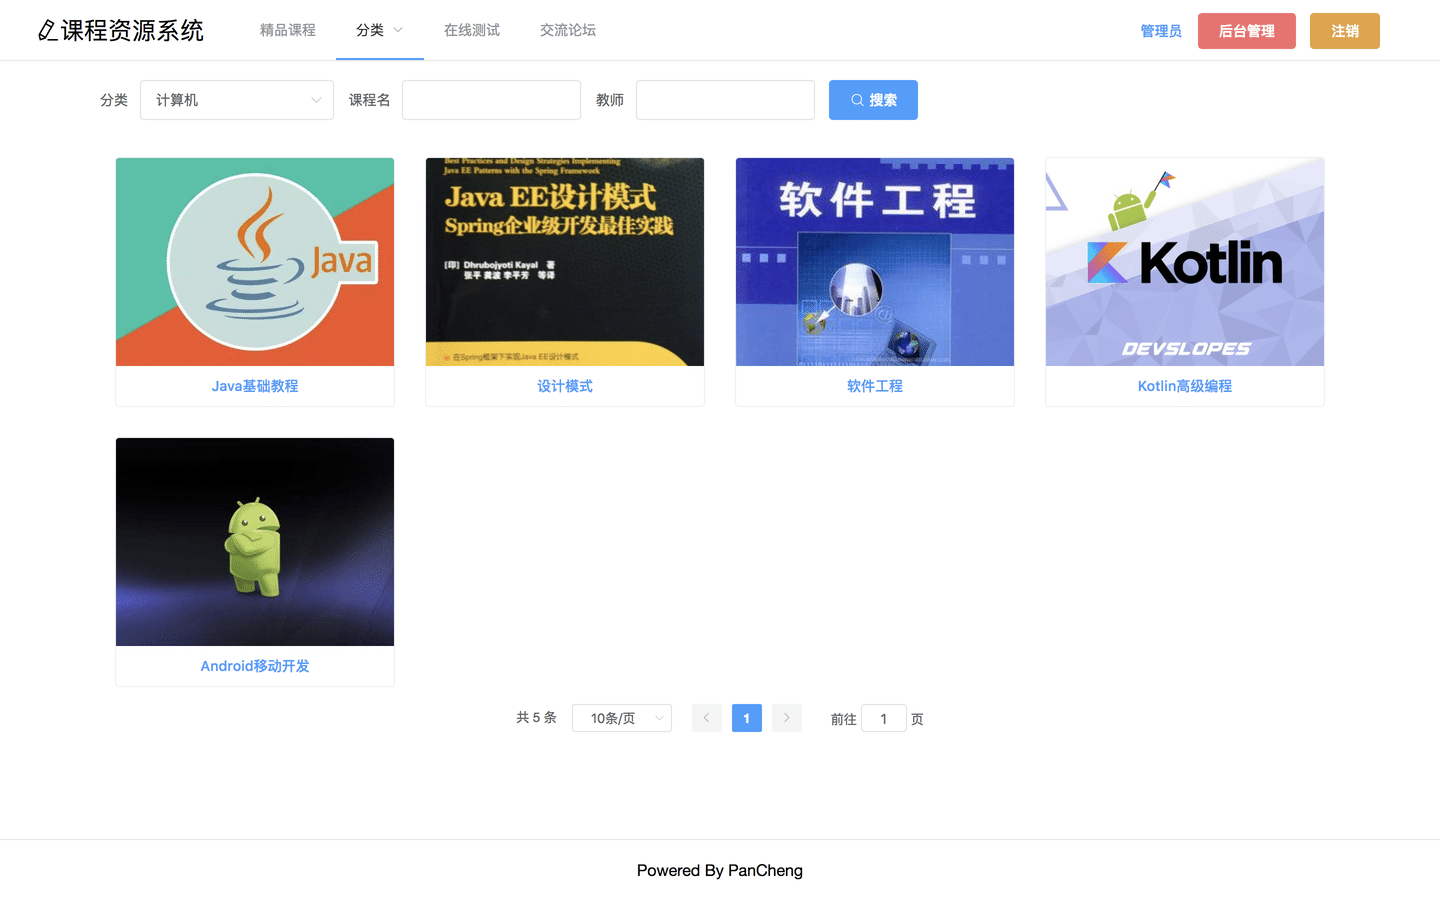
\includegraphics[width=140mm]{view-course-list.png}
    \caption{课程列表页}
    \label{fig:view-course-list}
\end{figure}
\begin{figure}[H]
    \centering
    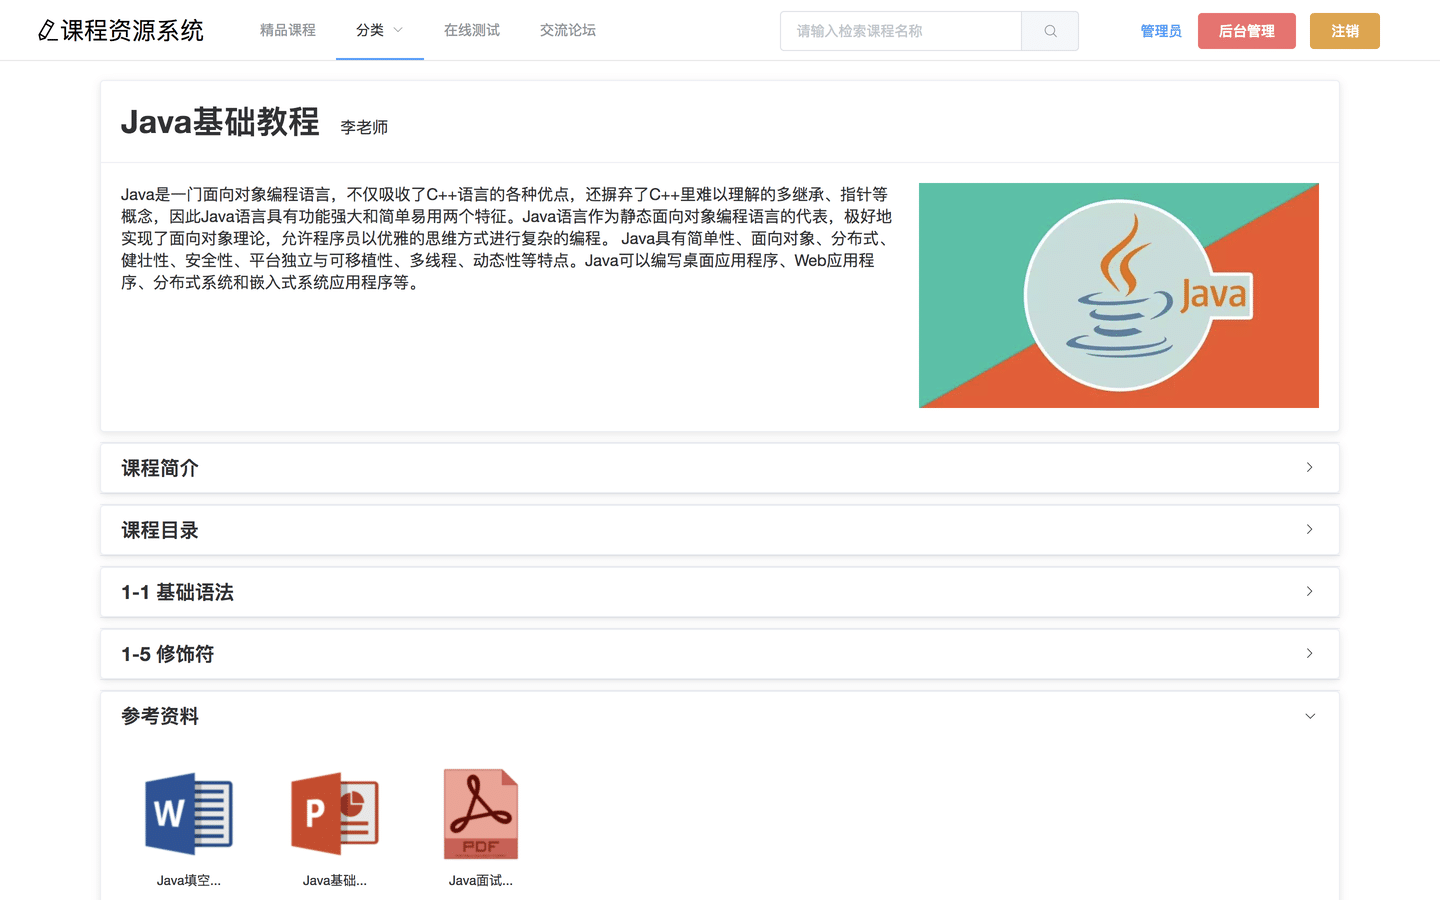
\includegraphics[width=140mm]{view-course.png}
    \caption{课程详情页}
    \label{fig:view-course}
\end{figure}
\begin{figure}[H]
    \centering
    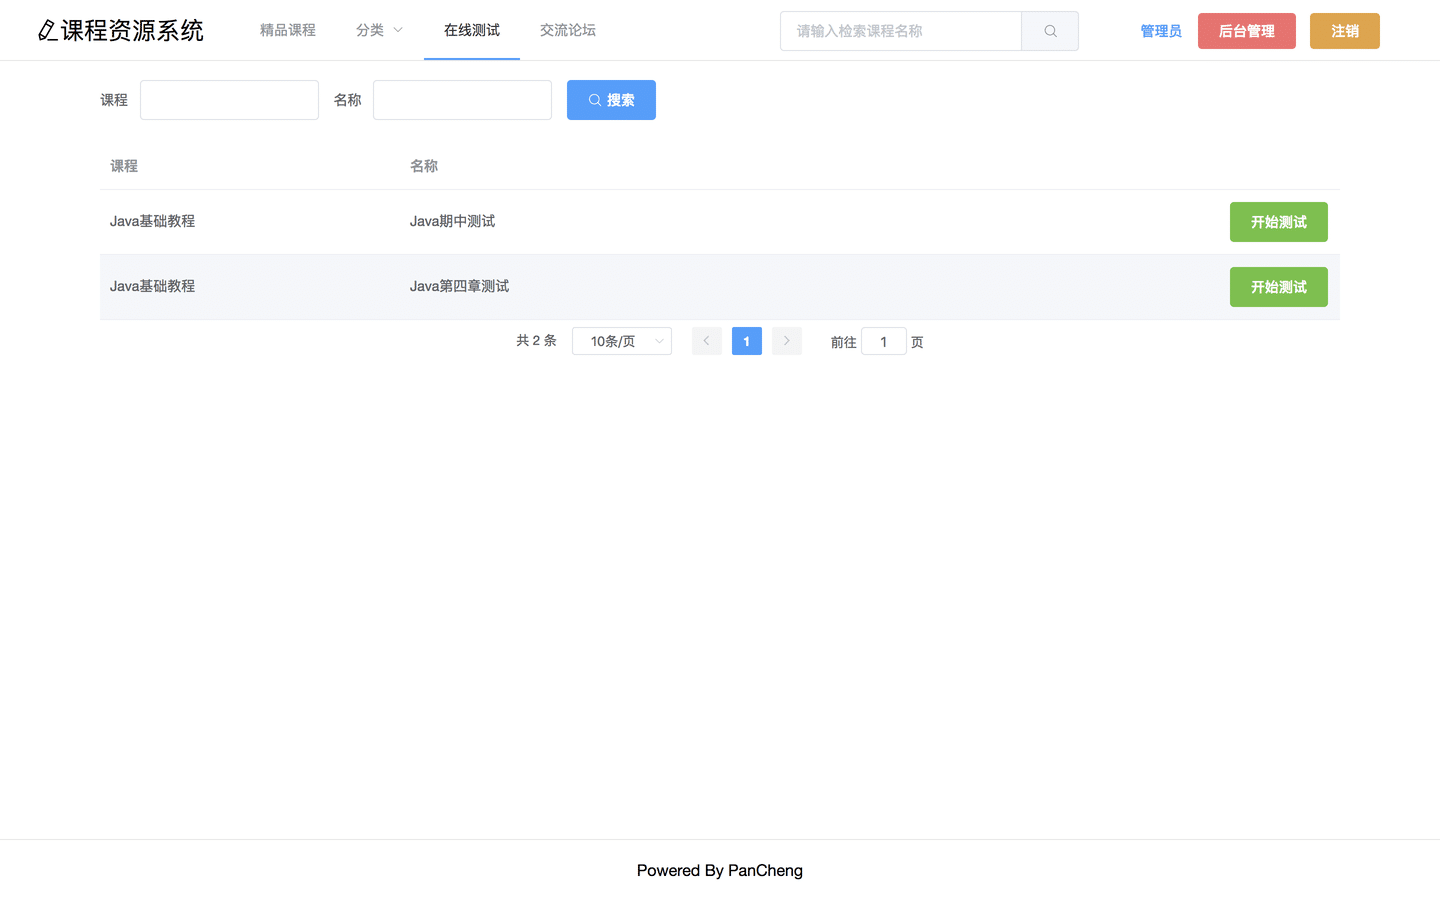
\includegraphics[width=140mm]{view-exam-list.png}
    \caption{在线测试列表页}
    \label{fig:view-exam-list}
\end{figure}
\begin{figure}[H]
    \centering
    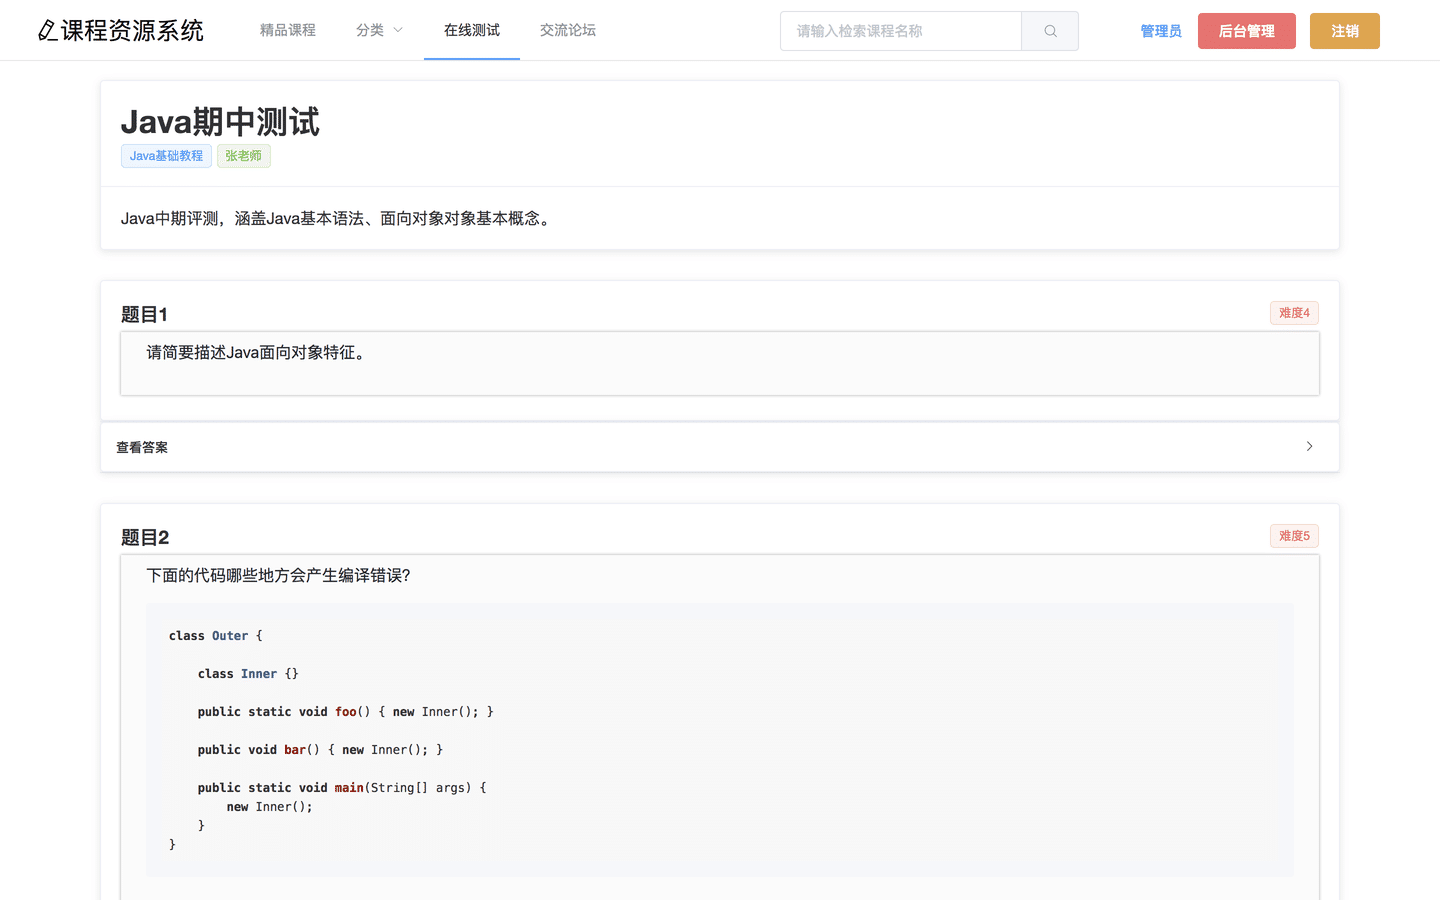
\includegraphics[width=140mm]{view-exam.png}
    \caption{在线测试详情页}
    \label{fig:view-exam}
\end{figure}
\begin{figure}[H]
    \centering
    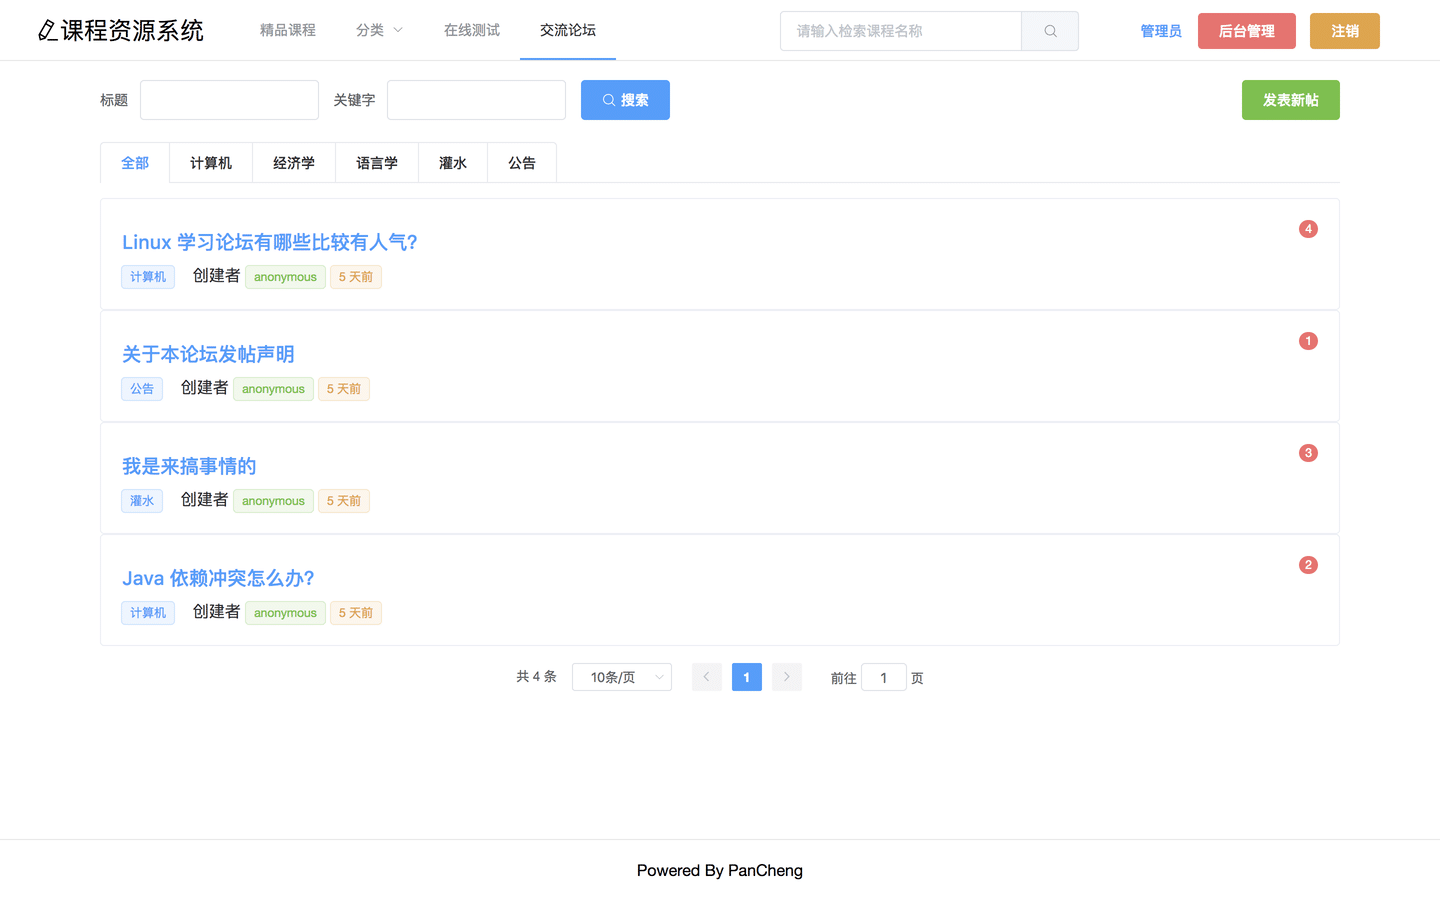
\includegraphics[width=140mm]{view-forum.png}
    \caption{论坛页}
    \label{fig:view-forum}
\end{figure}
\begin{figure}[H]
    \centering
    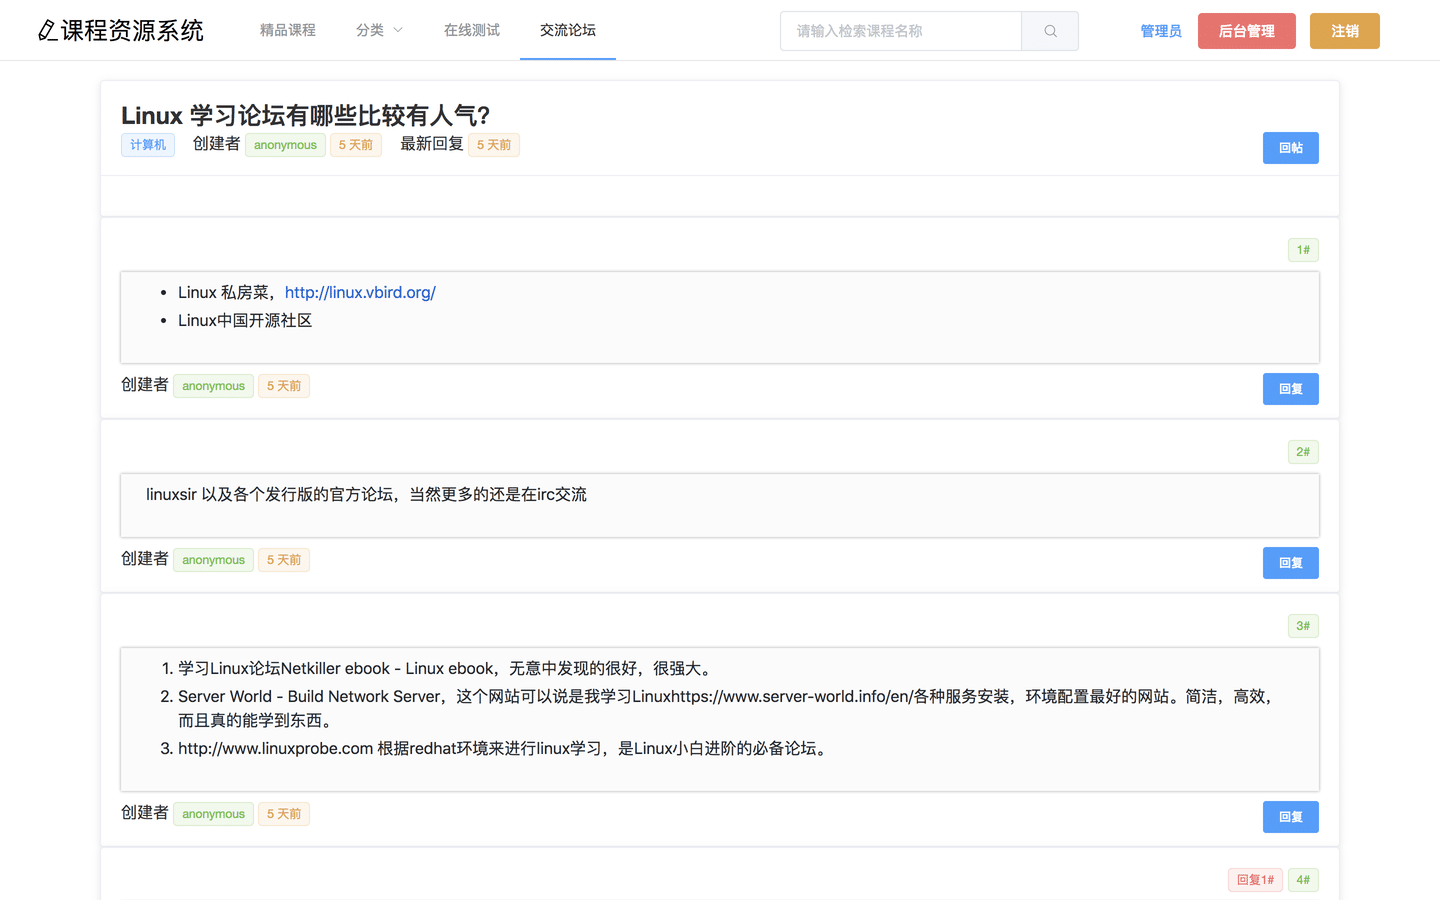
\includegraphics[width=140mm]{view-topic.png}
    \caption{帖子页}
    \label{fig:view-topic}
\end{figure}

\subsubsection{后台管理界面}
\begin{figure}[H]
    \centering
    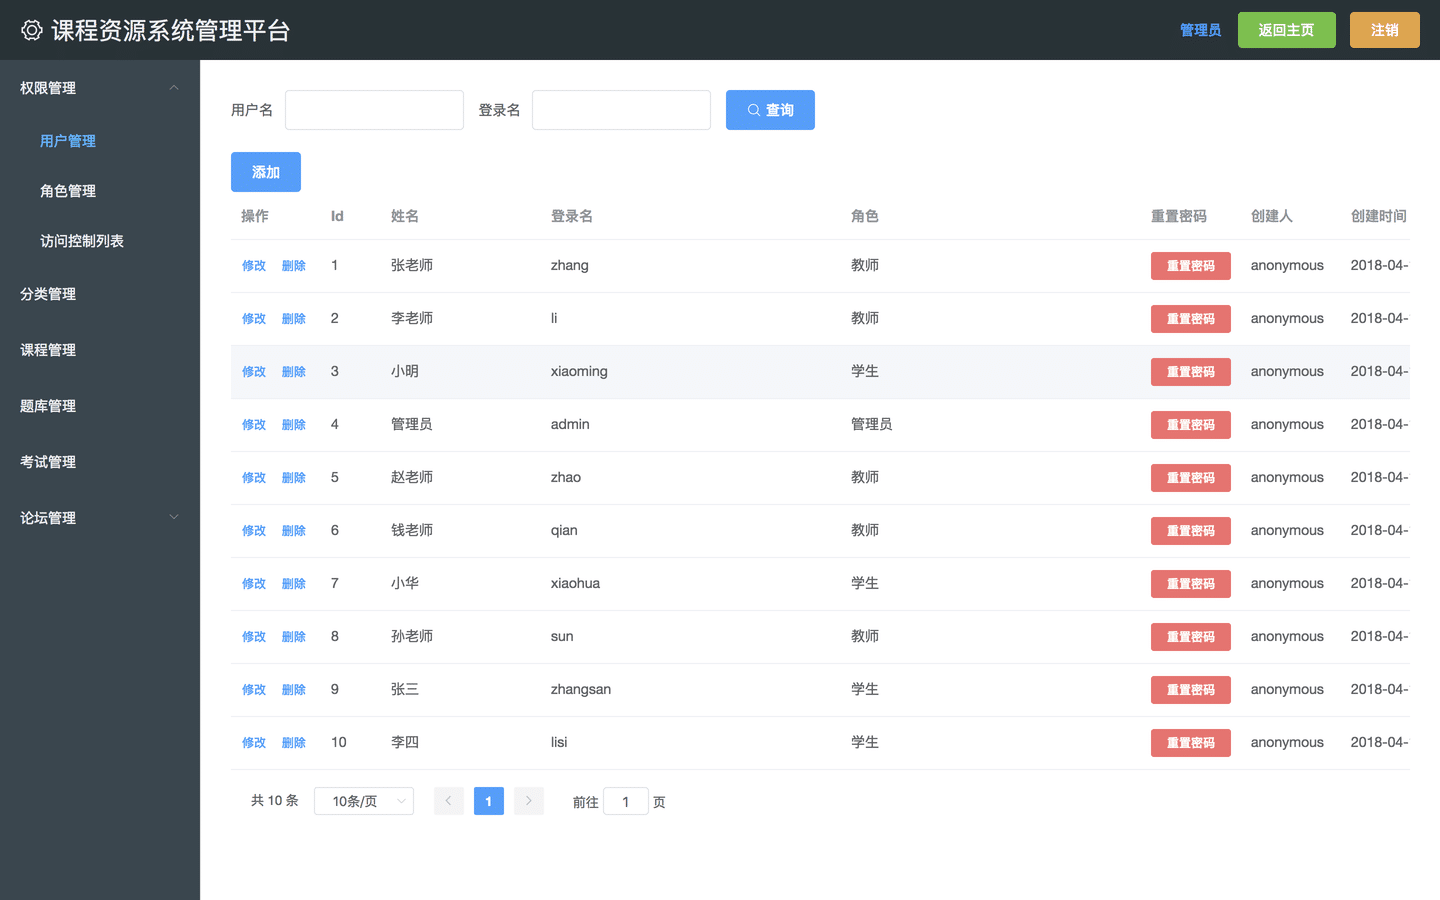
\includegraphics[width=140mm]{view-user-admin.png}
    \caption{用户管理页}
    \label{fig:view-user-admin}
\end{figure}
\begin{figure}[H]
    \centering
    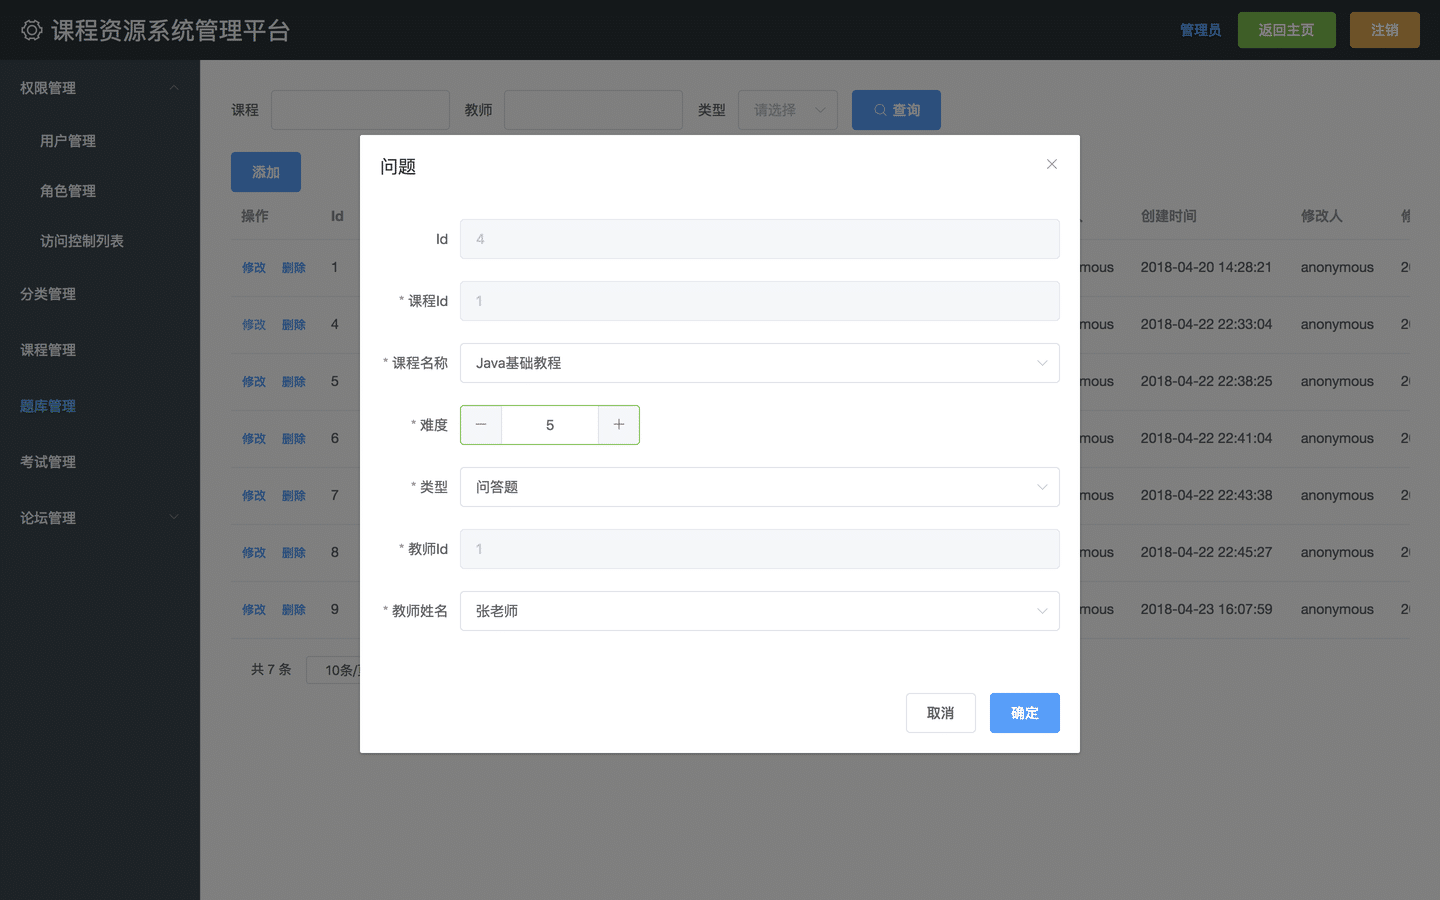
\includegraphics[width=140mm]{view-question-admin.png}
    \caption{问题管理页}
    \label{fig:view-question-admin}
\end{figure}

\subsection{系统交互接口}
\subsubsection{接口请求规范}
本系统所有微服务对外提供调用接口均为HTTP协议接口,接口参考RESTful风格设计,尽可能使用HTTP语义动作。常规资源的增删改查接口如表
\ref{tab:api}所示。\par
\begin{longtable}{|p{5em}|p{10em}|p{10em}|p{10em}|}
    \caption{微服务接口}\label{tab:api}                                        \\\hline
    HTTP方法 & URL                   & 参数               & 语义               \\\hline
    \endfirsthead
    \multicolumn{4}{r}{{续\tablename\thetable{}}}                              \\\hline
    \endhead
    GET      & /api/{资源类目}       & 无                 & 获取资源列表       \\\hline
    GET      & /api/{资源类目}/{id}  & 无                 & 获取指定资源       \\\hline
    POST     & /api/{资源类目}/query & 查询条件(JSON)     & 根据条件检索资源   \\\hline
    POST     & /api/{资源类目}       & 资源对象实体(JSON) & 新增或更新指定资源 \\\hline
    DELETE   & /api/{资源类目}/{id}  & 无                 & 删除指定资源       \\\hline
\end{longtable}
除常规的资源增删改查外,其余交互动作根据具体语义参考RESTful规范确定HTTP方法,URL以及参数。\par

\subsubsection{接口返回规范}
微服务接口返回数据统一使用JSON序列化,包含表\ref{tab:rest-result}字段。\par
\begin{longtable}{|p{10em}|p{10em}|p{10em}|}
    \caption{微服务接口返回数据结构}\label{tab:rest-result} \\\hline
    字段 & 类型   & 说明                                    \\\hline
    \endfirsthead
    \multicolumn{3}{r}{{续\tablename\thetable{}}}           \\\hline
    \endhead
    code & Int    & 标识码                                  \\\hline
    msg  & String & 消息说明                                \\\hline
    data & Any    & 返回数据                                \\\hline
    meta & Any    & 元数据                                  \\\hline
\end{longtable}

\subsection{系统出错处理}
若微服务接口调用出错,在服务器打印异常堆栈日志,并根据接口返回规范返回指定的标识码并携带简要的异常信息。标识码定义如表
\ref{tab:rest-result-code}所示。\par
\begin{longtable}{|p{15em}|p{5em}|p{10em}|}
    \caption{微服务接口标识码定义列表}\label{tab:rest-result-code} \\\hline
    名称                 & 标识码 & 说明                           \\\hline
    \endfirsthead
    \multicolumn{3}{r}{{续\tablename\thetable{}}}                  \\\hline
    \endhead
    SUCCESS\_CODE        & 1      & 操作成功                       \\\hline
    FAILURE\_CODE        & 0      & 操作失败                       \\\hline
    TOKEN\_INVALID\_CODE & 401    & 身份无效                       \\\hline
    NO\_PERMISSION\_CODE & 444    & 无权操作                       \\\hline
\end{longtable}

\clearpage

\section{数据库设计}
\subsection{概述}
本系统的持久化存储使用共两种数据库——关系型数据库MySQL,以及非关系型数据库Redis。\par
MySQL是当前互联网中最流行的关系型数据库管理系统,其小巧灵活的设计、免费开源的授权方式、优异的性能、以及良好的扩展性使得其广受欢迎,成为
关系型数据库中的佼佼者。数据作为应用的血液,数据存储应追求高度的可靠性和稳定性,MySQL最新发行版为8.0,发行时间为2018年4月20日,根据软
件行业经验,一般在MySQL新版本发布至少一年以上,才用于生产环境。本系统为追求数据存储的稳定性,使用上一个稳定版本5.7,该版本目前已被广泛
采用,稳定性得到保证。MySQL部署环境为Ubuntu Linux Server 16.04 x64。\par
随着软件行业的发展和需求场景的日益多样化,使得原有的关系型数据库已不能完全满足需求,非关系型数据库(NoSQL)理念应运而生。Redis是NoSQL
阵营一个强有力的代表,它是一个基于内存的高速数据库,丰富的数据结构、灵活的模式、高速的读写速度使得其特别适用于缓存、高速队列等业务场景,
本应中用户Session信息读写最为频繁,正符合Redis所擅长的业务场景,故使用其作为用户登录Session池。本系统使用Redis3.0版本,部署环境为
Ubuntu Linux Server 16.04 x64。\par

\subsection{设计规范}
\subsubsection{MySQL规范}
根据工程实践经验,大型系统的性能瓶颈主要在数据库上,故在设计初应尽可能减小数据库的压力,按照具体业务分库分表,允许一定的字段冗余和反模式
设计。结合MySQL 5.7的具体特性,数据库使用InnoDB引擎,不在数据库表中定义外键,其关联关系在应用层手动控制,为保证业务逻辑的完整性,禁用
数据库存储过程和函数,将所有业务逻辑在应用层实现。\par
数据表采用BIGINT类型(对应Java或Kotlin中Long类型)自增长主键,每张表中包含id、create\_time、creator、modify\_time、modifier、
note、version字段。其中create\_time、creator、modify\_time、modifier由应用层框架在数据库时自动控制;note字段用于数据记录特殊
备注标识;version字段用于乐观锁,由框架自动控制,不手动修改。\par
对有频繁查询要求的字段,合理使用索引。慎用聚合索引,聚合索引字段不允许超过3个。\par
为保证系统的横向扩展型,每个微服务的数据库应独立,不允许微服务跨库调用。\par
\subsubsection{Redis规范}
Redis是基于内存的高速数据库,在意外断电时无法保证数据完整性,故在Redis中不保存对完整性有要求的数据。\par
Redis中所有数据均存储在内存中,存储空间有限,存储代价较高,数据要根据需求设定合理的过期时间或过期策略。\par

\subsection{总体设计}
依照数据库设计规范,每个微服务数据库独立,故数据库设计切分为4个模块,分别为权限模块,课程资源与在线测试模块,论坛模块,文件模块。\par
\subsubsection{E-R图}
\paragraph{权限模块}
\begin{figure}[H]
    \centering
    
\includegraphics[width=140mm]{er-auth.png}
    \caption{权限模块E-R图}
    \label{fig:er-auth}
\end{figure}
\paragraph{课程资源、在线测试、文件模块}
\begin{figure}[H]
    \centering
    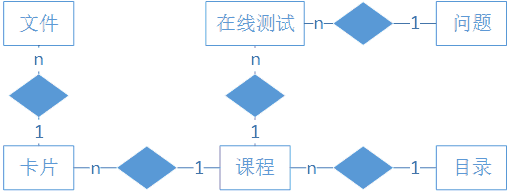
\includegraphics[width=100mm]{er-course-exam-file.png}
    \caption{课程资源、在线测试、文件模块E-R图}
    \label{fig:er-course-exam-file}
\end{figure}
\paragraph{论坛模块}
\begin{figure}[H]
    \centering
    
\includegraphics[width=140mm]{er-forum.png}
    \caption{论坛模块E-R图}
    \label{fig:er-forum}
\end{figure}

\subsection{具体设计}
\subsubsection{权限模块}
\paragraph{用户表user}
\subparagraph{实体图}
\begin{figure}[H]
    \centering
    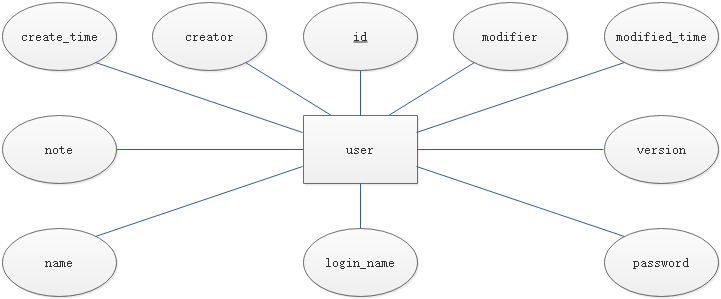
\includegraphics[width=140mm]{entity-user.png}
    \caption{用户实体图}
    \label{fig:entity-user}
\end{figure}
\subparagraph{字段表}
\begin{longtable}{|p{10em}|p{6em}|p{15em}|}
    \caption{用户user字段表}\label{tab:table_user}       \\\hline
    字段名         & 类型         & 说明                 \\\hline
    \endfirsthead
    \multicolumn{3}{r}{{续\tablename\thetable{}}}        \\\hline
    \endhead
    id             & bigint(20)   & 主键                 \\\hline
    name           & varchar(255) & 姓名                 \\\hline
    login\_name    & varchar(255) & 登录名               \\\hline
    password       & varchar(255) & 密码                 \\\hline
    creator        & varchar(255) & 创建人               \\\hline
    create\_time   & datetime(6)  & 创建时间             \\\hline
    modifier       & varchar(255) & 修改人               \\\hline
    modified\_time & datetime(6)  & 修改时间             \\\hline
    note           & text         & 备注                 \\\hline
    version        & bigint(20)   & 版本号(用于乐观锁) \\\hline
\end{longtable}\par

\paragraph{角色表role}
\subparagraph{实体图}
\begin{figure}[H]
    \centering
    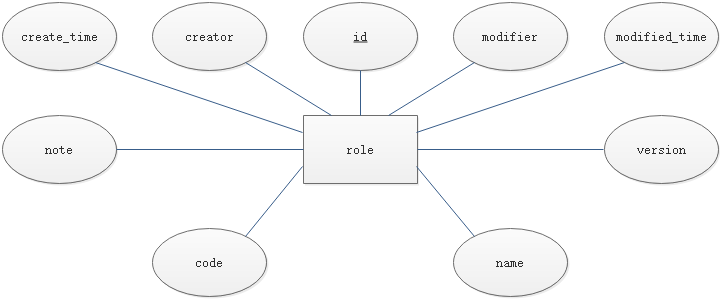
\includegraphics[width=140mm]{entity-role.png}
    \caption{角色实体图}
    \label{fig:entity-role}
\end{figure}
\subparagraph{字段表}
\begin{longtable}{|p{10em}|p{6em}|p{15em}|}
    \caption{角色role字段表}\label{tab:table_role}       \\\hline
    字段名         & 类型         & 说明                 \\\hline
    \endfirsthead
    \multicolumn{3}{r}{{续\tablename\thetable{}}}        \\\hline
    \endhead
    id             & bigint(20)   & 主键                 \\\hline
    code           & varchar(255) & 编码                 \\\hline
    name           & varchar(255) & 名称                 \\\hline
    creator        & varchar(255) & 创建人               \\\hline
    create\_time   & datetime(6)  & 创建时间             \\\hline
    modifier       & varchar(255) & 修改人               \\\hline
    modified\_time & datetime(6)  & 修改时间             \\\hline
    note           & text         & 备注                 \\\hline
    version        & bigint(20)   & 版本号(用于乐观锁) \\\hline
\end{longtable}\par

\paragraph{用户-角色关联表user\_role}
\subparagraph{实体图}
\begin{figure}[H]
    \centering
    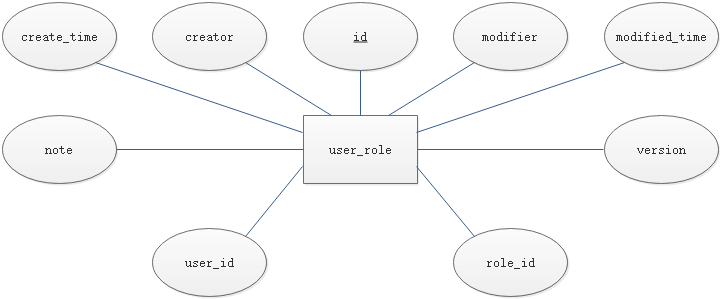
\includegraphics[width=140mm]{entity-user-role.png}
    \caption{用户-角色关联实体图}
    \label{fig:entity-user-role}
\end{figure}
\subparagraph{字段表}
\begin{longtable}{|p{10em}|p{6em}|p{15em}|}
    \caption{用户-角色关联user\_role字段表}\label{tab:table_user_role} \\\hline
    字段名         & 类型         & 说明                               \\\hline
    \endfirsthead
    \multicolumn{3}{r}{{续\tablename\thetable{}}}                      \\\hline
    \endhead
    id             & bigint(20)   & 主键                               \\\hline
    role\_id       & bigint(20)   & 关联role主键                       \\\hline
    user\_id       & bigint(20)   & 关联user主键                       \\\hline
    creator        & varchar(255) & 创建人                             \\\hline
    create\_time   & datetime(6)  & 创建时间                           \\\hline
    modifier       & varchar(255) & 修改人                             \\\hline
    modified\_time & datetime(6)  & 修改时间                           \\\hline
    note           & text         & 备注                               \\\hline
    version        & bigint(20)   & 版本号(用于乐观锁)               \\\hline
\end{longtable}\par

\paragraph{访问控制列表表acl}
\subparagraph{实体图}
\begin{figure}[H]
    \centering
    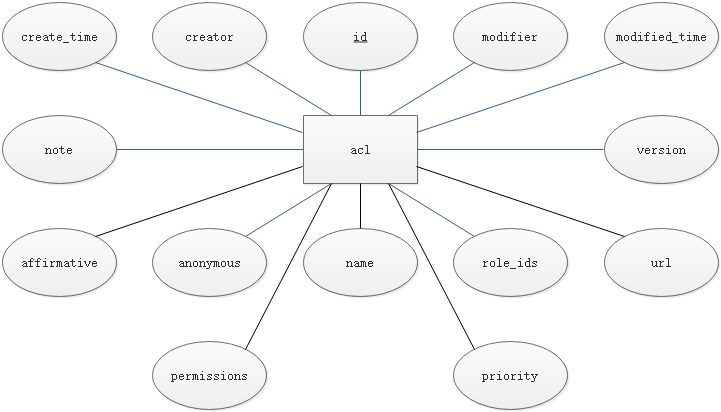
\includegraphics[width=140mm]{entity-acl.png}
    \caption{访问控制列表实体图}
    \label{fig:entity-acl}
\end{figure}
\subparagraph{字段表}
\begin{longtable}{|p{10em}|p{6em}|p{15em}|}
    \caption{访问控制列表acl字段表}\label{tab:table_acl}   \\\hline
    字段名         & 类型         & 说明                   \\\hline
    \endfirsthead
    \multicolumn{3}{r}{{续\tablename\thetable{}}}          \\\hline
    \endhead
    id             & bigint(20)   & 主键                   \\\hline
    affirmative    & bit(1)       & 高级授权标志位         \\\hline
    anonymous      & bit(1)       & 允许匿名标志位         \\\hline
    permissions    & varchar(255) & 权限表详情(扩展保留) \\\hline
    priority       & int(11)      & 优先级(数值小优先)   \\\hline
    role\_ids      & varchar(255) & 关联role主键集合       \\\hline
    url            & text         & 匹配URL模板            \\\hline
    creator        & varchar(255) & 创建人                 \\\hline
    create\_time   & datetime(6)  & 创建时间               \\\hline
    modifier       & varchar(255) & 修改人                 \\\hline
    modified\_time & datetime(6)  & 修改时间               \\\hline
    note           & text         & 备注                   \\\hline
    version        & bigint(20)   & 版本号(用于乐观锁)   \\\hline
\end{longtable}\par

\subsubsection{课程资源与在线测试模块}
\paragraph{分类表category}
\subparagraph{实体图}
\begin{figure}[H]
    \centering
    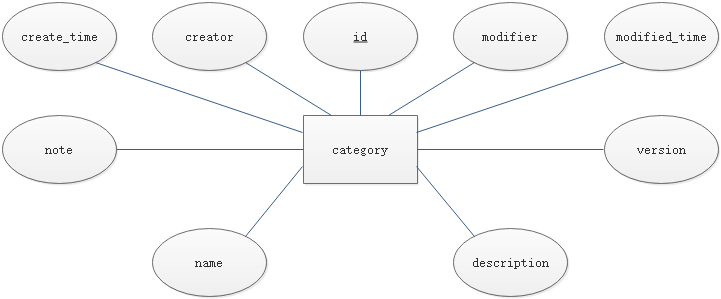
\includegraphics[width=140mm]{entity-category.png}
    \caption{分类实体图}
    \label{fig:entity-category}
\end{figure}
\subparagraph{字段表}
\begin{longtable}{|p{10em}|p{6em}|p{15em}|}
    \caption{分类category字段表}\label{tab:table_category} \\\hline
    字段名         & 类型         & 说明                   \\\hline
    \endfirsthead
    \multicolumn{3}{r}{{续\tablename\thetable{}}}          \\\hline
    \endhead
    id             & bigint(20)   & 主键                   \\\hline
    name           & varchar(255) & 名称                   \\\hline
    description    & text         & 描述                   \\\hline
    creator        & varchar(255) & 创建人                 \\\hline
    create\_time   & datetime(6)  & 创建时间               \\\hline
    modifier       & varchar(255) & 修改人                 \\\hline
    modified\_time & datetime(6)  & 修改时间               \\\hline
    note           & text         & 备注                   \\\hline
    version        & bigint(20)   & 版本号(用于乐观锁)   \\\hline
\end{longtable}\par

\paragraph{卡片表card}
\subparagraph{实体图}
\begin{figure}[H]
    \centering
    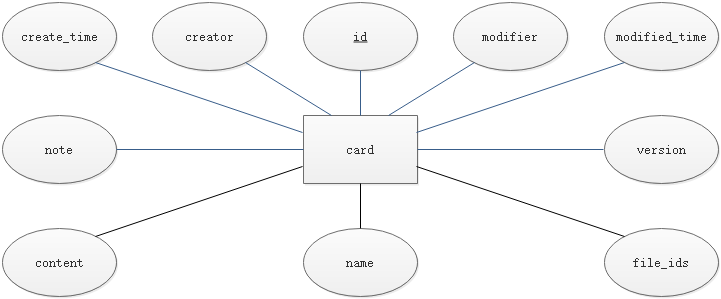
\includegraphics[width=140mm]{entity-card.png}
    \caption{卡片实体图}
    \label{fig:entity-card}
\end{figure}
\subparagraph{字段表}
\begin{longtable}{|p{10em}|p{6em}|p{15em}|}
    \caption{卡片card字段表}\label{tab:table_card}       \\\hline
    字段名         & 类型         & 说明                 \\\hline
    \endfirsthead
    \multicolumn{3}{r}{{续\tablename\thetable{}}}        \\\hline
    \endhead
    id             & bigint(20)   & 主键                 \\\hline
    name           & varchar(255) & 名称                 \\\hline
    file\_ids      & varchar(255) & 关联file主键集合     \\\hline
    content        & text         & 内容(markdown文本) \\\hline
    creator        & varchar(255) & 创建人               \\\hline
    create\_time   & datetime(6)  & 创建时间             \\\hline
    modifier       & varchar(255) & 修改人               \\\hline
    modified\_time & datetime(6)  & 修改时间             \\\hline
    note           & text         & 备注                 \\\hline
    version        & bigint(20)   & 版本号(用于乐观锁) \\\hline
\end{longtable}\par

\paragraph{课程表course}
\subparagraph{实体图}
\begin{figure}[H]
    \centering
    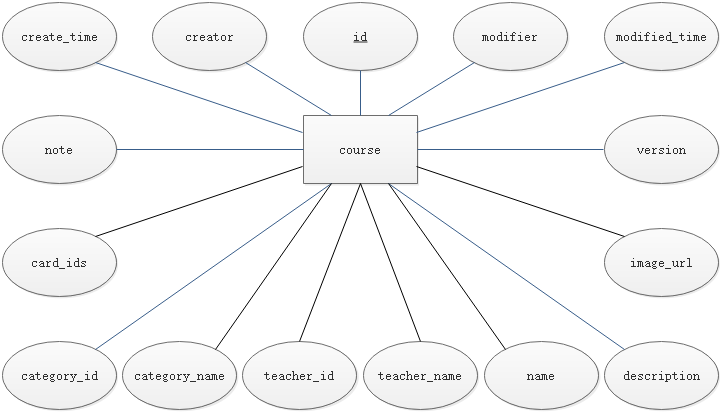
\includegraphics[width=140mm]{entity-course.png}
    \caption{课程实体图}
    \label{fig:entity-course}
\end{figure}
\subparagraph{字段表}
\begin{longtable}{|p{10em}|p{6em}|p{15em}|}
    \caption{课程course字段表}\label{tab:table_course}   \\\hline
    字段名         & 类型         & 说明                 \\\hline
    \endfirsthead
    \multicolumn{3}{r}{{续\tablename\thetable{}}}        \\\hline
    \endhead
    id             & bigint(20)   & 主键                 \\\hline
    name           & varchar(255) & 名称                 \\\hline
    description    & text         & 描述                 \\\hline
    card\_ids      & varchar(255) & 关联card主键集合     \\\hline
    category\_id   & bigint(20)   & 关联category主键     \\\hline
    category\_name & varchar(255) & 关联category名称     \\\hline
    teacher\_id    & bigint(20)   & 教师id               \\\hline
    teacher\_name  & varchar(255) & 教师姓名             \\\hline
    image\_url     & text         & 图片链接             \\\hline
    creator        & varchar(255) & 创建人               \\\hline
    create\_time   & datetime(6)  & 创建时间             \\\hline
    modifier       & varchar(255) & 修改人               \\\hline
    modified\_time & datetime(6)  & 修改时间             \\\hline
    note           & text         & 备注                 \\\hline
    version        & bigint(20)   & 版本号(用于乐观锁) \\\hline
\end{longtable}\par

\paragraph{问题表question}
\subparagraph{实体图}
\begin{figure}[H]
    \centering
    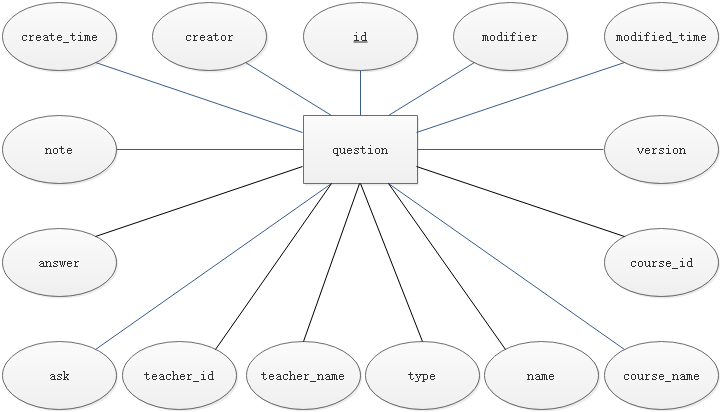
\includegraphics[width=140mm]{entity-question.png}
    \caption{问题实体图}
    \label{fig:entity-question}
\end{figure}
\subparagraph{字段表}
\begin{longtable}{|p{10em}|p{6em}|p{15em}|}
    \caption{问题question字段表}\label{tab:table_question} \\\hline
    字段名         & 类型          & 说明                  \\\hline
    \endfirsthead
    \multicolumn{3}{r}{{续\tablename\thetable{}}}          \\\hline
    \endhead
    id             & bigint(20)    & 主键                  \\\hline
    course\_id     & bigint(20)    & 关联course主键        \\\hline
    course\_name   & varchar(255)  & 关联course名称        \\\hline
    teacher\_id    & bigint(20)    & 教师id                \\\hline
    teacher\_name  & varchar(255)  & 教师姓名              \\\hline
    ask            & text          & 题目(markdown文本)    \\\hline
    anwser         & text          & 答案(markdown文本)    \\\hline
    score          & decimal(19,2) & 分值(难度)          \\\hline
    type           & varchar(255)  & 类型                  \\\hline
    creator        & varchar(255)  & 创建人                \\\hline
    create\_time   & datetime(6)   & 创建时间              \\\hline
    modifier       & varchar(255)  & 修改人                \\\hline
    modified\_time & datetime(6)   & 修改时间              \\\hline
    note           & text          & 备注                  \\\hline
    version        & bigint(20)    & 版本号(用于乐观锁)  \\\hline
\end{longtable}\par

\paragraph{考试表exam}
\subparagraph{实体图}
\begin{figure}[H]
    \centering
    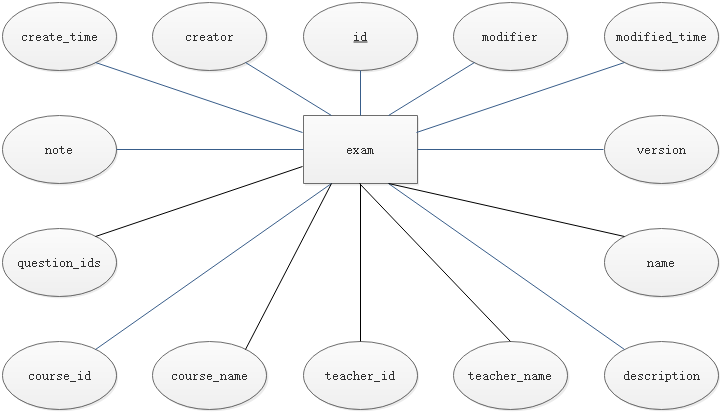
\includegraphics[width=140mm]{entity-exam.png}
    \caption{考试实体图}
    \label{fig:entity-exam}
\end{figure}
\subparagraph{字段表}
\begin{longtable}{|p{10em}|p{6em}|p{15em}|}
    \caption{考试exam字段表}\label{tab:table_exam}       \\\hline
    字段名         & 类型         & 说明                 \\\hline
    \endfirsthead
    \multicolumn{3}{r}{{续\tablename\thetable{}}}        \\\hline
    \endhead
    id             & bigint(20)   & 主键                 \\\hline
    name           & varchar(255) & 名称                 \\\hline
    description    & text         & 描述                 \\\hline
    course\_id     & bigint(20)   & 关联course主键       \\\hline
    course\_name   & varchar(255) & 关联course名称       \\\hline
    teacher\_id    & bigint(20)   & 教师id               \\\hline
    teacher\_name  & varchar(255) & 教师姓名             \\\hline
    creator        & varchar(255) & 创建人               \\\hline
    create\_time   & datetime(6)  & 创建时间             \\\hline
    modifier       & varchar(255) & 修改人               \\\hline
    modified\_time & datetime(6)  & 修改时间             \\\hline
    note           & text         & 备注                 \\\hline
    version        & bigint(20)   & 版本号(用于乐观锁) \\\hline
\end{longtable}\par

\subsubsection{论坛模块}
\paragraph{板块表block}
\subparagraph{实体图}
\begin{figure}[H]
    \centering
    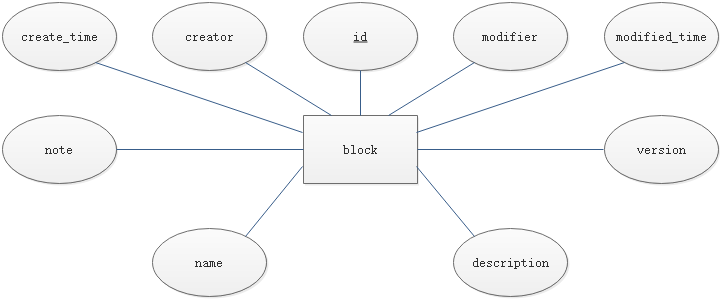
\includegraphics[width=140mm]{entity-block.png}
    \caption{板块实体图}
    \label{fig:entity-block}
\end{figure}
\subparagraph{字段表}
\begin{longtable}{|p{10em}|p{6em}|p{15em}|}
    \caption{板块block字段表}\label{tab:table_block}     \\\hline
    字段名         & 类型         & 说明                 \\\hline
    \endfirsthead
    \multicolumn{3}{r}{{续\tablename\thetable{}}}        \\\hline
    \endhead
    id             & bigint(20)   & 主键                 \\\hline
    name           & varchar(255) & 名称                 \\\hline
    description    & text         & 描述                 \\\hline
    creator        & varchar(255) & 创建人               \\\hline
    create\_time   & datetime(6)  & 创建时间             \\\hline
    modifier       & varchar(255) & 修改人               \\\hline
    modified\_time & datetime(6)  & 修改时间             \\\hline
    note           & text         & 备注                 \\\hline
    version        & bigint(20)   & 版本号(用于乐观锁) \\\hline
\end{longtable}\par

\paragraph{发言表discussion}
\subparagraph{实体图}
\begin{figure}[H]
    \centering
    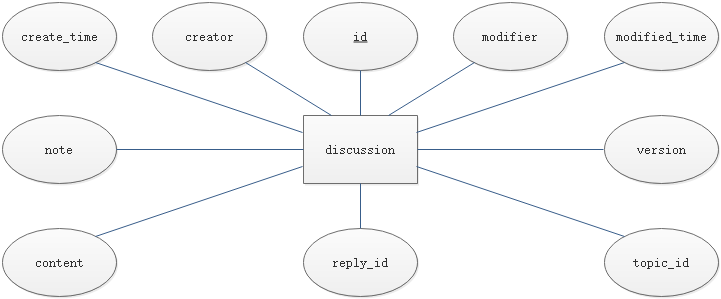
\includegraphics[width=140mm]{entity-discussion.png}
    \caption{发言实体图}
    \label{fig:entity-discussion}
\end{figure}
\subparagraph{字段表}
\begin{longtable}{|p{10em}|p{6em}|p{15em}|}
    \caption{发言discussion字段表}\label{tab:table_discussion} \\\hline
    字段名         & 类型         & 说明                       \\\hline
    \endfirsthead
    \multicolumn{3}{r}{{续\tablename\thetable{}}}              \\\hline
    \endhead
    id             & bigint(20)   & 主键                       \\\hline
    topic\_id      & bigint(20)   & 关联topic主键              \\\hline
    reply\_id      & bigint(20)   & 回复discussion主键         \\\hline
    content        & mediumtext   & 内容(markdown文本)       \\\hline
    creator        & varchar(255) & 创建人                     \\\hline
    create\_time   & datetime(6)  & 创建时间                   \\\hline
    modifier       & varchar(255) & 修改人                     \\\hline
    modified\_time & datetime(6)  & 修改时间                   \\\hline
    note           & text         & 备注                       \\\hline
    version        & bigint(20)   & 版本号(用于乐观锁)       \\\hline
\end{longtable}\par

\paragraph{话题表topic}
\subparagraph{实体图}
\begin{figure}[H]
    \centering
    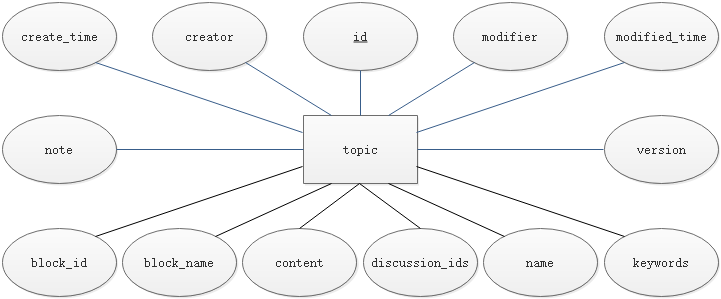
\includegraphics[width=140mm]{entity-topic.png}
    \caption{话题实体图}
    \label{fig:entity-topic}
\end{figure}
\subparagraph{字段表}
\begin{longtable}{|p{10em}|p{6em}|p{15em}|}
    \caption{话题topic字段表}\label{tab:table_topic}        \\\hline
    字段名          & 类型         & 说明                   \\\hline
    \endfirsthead
    \multicolumn{3}{r}{{续\tablename\thetable{}}}           \\\hline
    \endhead
    id              & bigint(20)   & 主键                   \\\hline
    name            & varchar(255) & 标题                   \\\hline
    block\_id       & bigint(20)   & 关联block主键          \\\hline
    block\_name     & varchar(255) & 关联block名称          \\\hline
    content         & mediumtext   & 内容(markdown文本)   \\\hline
    discussion\_ids & varchar(255) & 关联discussion主键集合 \\\hline
    keywords        & varchar(255) & 关键词                 \\\hline
    creator         & varchar(255) & 创建人                 \\\hline
    create\_time    & datetime(6)  & 创建时间               \\\hline
    modifier        & varchar(255) & 修改人                 \\\hline
    modified\_time  & datetime(6)  & 修改时间               \\\hline
    note            & text         & 备注                   \\\hline
    version         & bigint(20)   & 版本号(用于乐观锁)   \\\hline
\end{longtable}\par

\subsubsection{文件模块}
\paragraph{文件表file}
\subparagraph{实体图}
\begin{figure}[H]
    \centering
    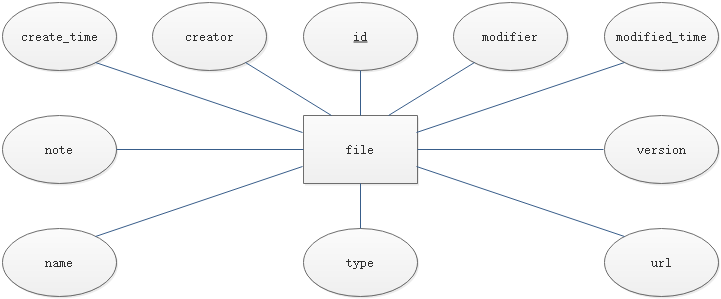
\includegraphics[width=140mm]{entity-file.png}
    \caption{文件实体图}
    \label{fig:entity-file}
\end{figure}
\subparagraph{字段表}
\begin{longtable}{|p{10em}|p{6em}|p{15em}|}
    \caption{文件表file字段表}\label{tab:table_file}     \\\hline
    字段名         & 类型         & 说明                 \\\hline
    \endfirsthead
    \multicolumn{3}{r}{{续\tablename\thetable{}}}        \\\hline
    \endhead
    id             & bigint(20)   & 主键                 \\\hline
    name           & varchar(255) & 文件名               \\\hline
    type           & varchar(255) & 文件类型             \\\hline
    url            & text         & 文件下载链接         \\\hline
    creator        & varchar(255) & 创建人               \\\hline
    create\_time   & datetime(6)  & 创建时间             \\\hline
    modifier       & varchar(255) & 修改人               \\\hline
    modified\_time & datetime(6)  & 修改时间             \\\hline
    note           & text         & 备注                 \\\hline
    version        & bigint(20)   & 版本号(用于乐观锁) \\\hline
\end{longtable}\par
\clearpage

\section{详细设计}
\subsection{分布式微服务架构}
\subsubsection{架构总览}
相比于传统的单体应用集众多功能于一身,分布式微服务将系统繁杂的功能切分成独立的功能,每个服务专注一个或几个功能的实现,
保证微服务内部的简单性。简单即可靠,微服务内部的简单性提高了微服务的可靠性,在整个系统中,即便单个服务的崩溃,亦不至于
导致整个系统的瘫痪。\par
\begin{figure}[H]
    \centering
    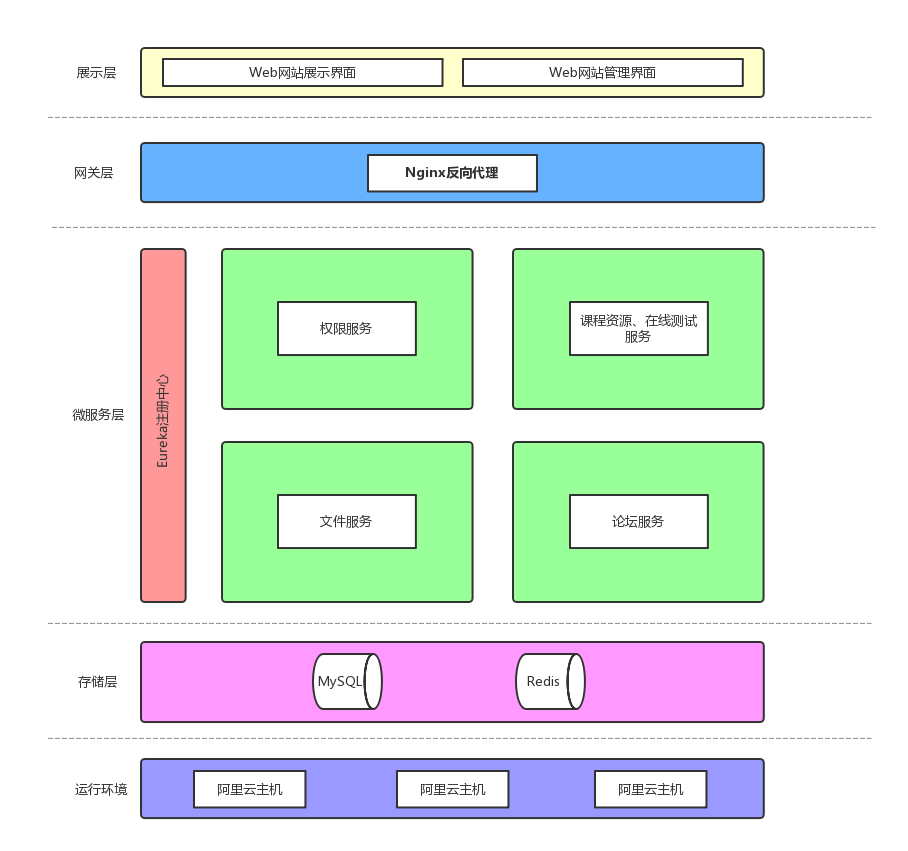
\includegraphics[width=150mm]{arch-overall.png}
    \caption{系统总架构图}
    \label{fig:arch-overall}
\end{figure}
\begin{figure}[H]
    \centering
    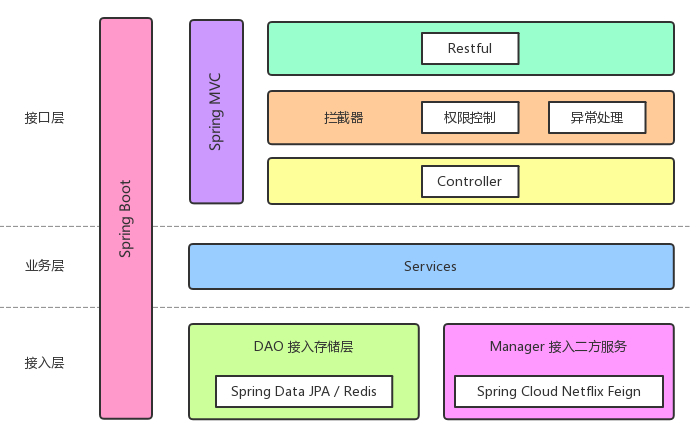
\includegraphics[width=150mm]{arch-microserver.png}
    \caption{微服务内部架构图}
    \label{fig:arch-microserver}
\end{figure}
本系统选择了较为前沿的Spring Cloud分布式微服务技术架构。Spring Cloud是一个基于Spring Boot实现的微服务开发框架,它为基于JVM开发的云应用中的
服务发现、断路器、微代理、配置管理、全局锁、智能路由、决策竞选、控制总线、集群状态管理和分布式会话等操作提供了一种简单的开发方式。\par
Spring Cloud集合了众多的开源项目,限于时间和精力,本项目仅采用了其中部分的功能。\par
\subsubsection{服务注册与发现}
在分布式微服务技术架构中,各个微服务间的通信是首先需要解决的问题,如果每个微服务手工指定其他服务的通信地址,随着应用的增多,配置代价将迅速提升,并且
当一个服务改变位置后,要重新配置依赖其的所有应用,可维护性极差。因此,这里使用微服务基于注册和发现的策略,所有微服务在启动后向服务注册中心注册,并从
注册中心查找依赖的其他微服务地址,以达到服务自动发现的目的。\par
服务注册与发现的思想,与Spring框架本身的核心概念控制反转有异曲同工之处。控制反转是Spring最核心的概念之一,是指将类以Bean的形式注册到Spring容器,
类之间协作只需声明依赖关系,不需要手工实例化,全权由Spring容器负责依赖注入和实例化装配,大大简化了Java EE的开发流程。从某种意义上来讲,服务注册与
发现思想是对控制反转思想的延伸。\par
在具体实现中,本系统用到了Spring Cloud Netflix模块中的Eureka模块。\par
\begin{figure}[H]
    \centering
    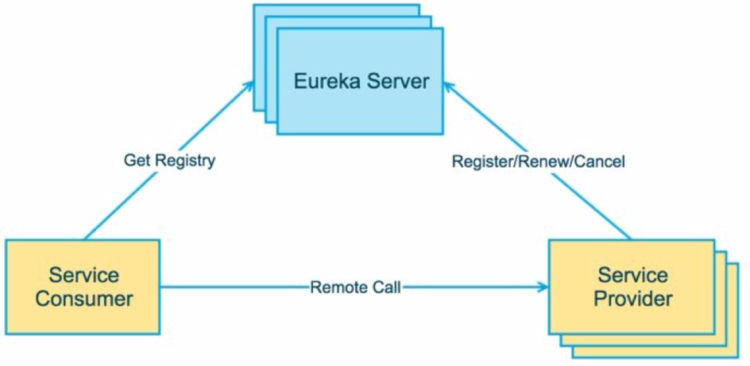
\includegraphics[width=130mm]{struct-eureka.png}
    \caption{Eureka注册中心服务发现}
    \label{fig:struct-eureka}
\end{figure}

\subsection{微服务间通信}
所有微服务暴露的外部调用接口均为RESTful风格的HTTP接口,其中生产者使用Spring MVC框架实现,消费者使用Spring Cloud OpenFeign框架实现。\par
\subsubsection{生产者}
Spring MVC是一套完整的MVC层开发框架,本系统中并不使用其View功能,仅仅通过Controller接受HTTP请求,并将结果渲染成JSON作为HTTP的Body数据返回。\par
其中,JSON的序列化与反序列化过程依赖Spring MVC框架中的HttpMessageConverter组件,其工作流程如图\ref{fig:flow-spring-mvc-rest}所示。本系统中
使用Spring Boot中Web模块的默认配置,即Jackson实现JSON的序列化与反序列化。\par
\begin{figure}[H]
    \centering
    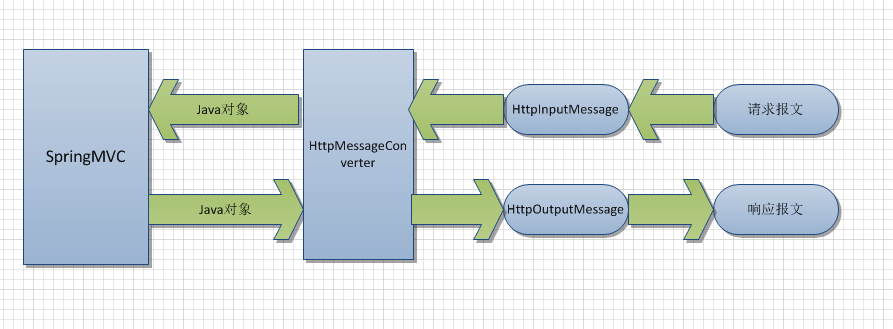
\includegraphics[width=150mm]{flow-spring-mvc-rest.png}
    \caption{JSON序列化与反序列化过程}
    \label{fig:flow-spring-mvc-rest}
\end{figure}
具体实现时,通过@RestController注解修饰Controller类,并将其所在包加入到Spring框架组件扫描范围,即可被Spring MVC框架自动识别。\par
\begin{mdframed}\begin{verbatim}
@RestController
@RequestMapping("/api/user")
class UserController(@Autowired override val service: UserService)
    : BaseController<UserDTO, UserDO, UserService>() {

    @Log
    @GetMapping("idNameList")
    fun getIdNameList(): RestResult {
        return successRestResult(service.fetchIdNameList())
    }
}
\end{verbatim}\end{mdframed}\par

\subsubsection{消费者}
Spring Cloud OpenFeign是Spring Cloud框架中的一个HTTP客户端代理组件,其仿造Spring MVC框架中Controller方法的风格,只需在类上添加
@FeignClient注解,并按照类似生产者的方式声明一个接口,即可由框架实现自动调用。\par
\begin{mdframed}\begin{verbatim}
@FeignClient(name = "crs-auth-server", path = "/api/client")
interface AuthManager {

    @PostMapping("/checkAnonymous")
    fun checkAnonymous(@RequestParam url: String): Boolean
}
\end{verbatim}\end{mdframed}\par
Feign仅仅是一个接口规范,其具体实现支持OkHttp3或Apache HttpClient两种方案,本系统采用Spring Boot的默认配置Apache HttpClient方案。\par
鉴于本系统中所有生产者接返回数据口均经过统一的包装,真正的数据存储在data字段,如果直接使用Feign默认的JSON反序列化器,则每个调用接口需要手动
拆包,获取data字段。为简化消费者的调用,这里重写Feign的解码器,若调用生产者接口返回报文code为SUCCESS\_CODE,则取出data字段,通过FastJson
反序列化成Kotlin对象返回给消费者,否则抛出异常。\par
\begin{mdframed}\begin{verbatim}
class CustomizedResponseEntityDecoder(decoder: Decoder)
    : ResponseEntityDecoder(decoder) {

  private val logger: Logger = LoggerFactory.getLogger(this.javaClass)

  override fun decode(response: Response, type: Type): Any {
    val restResult = super.decode(response, RestResult::class.java) 
            as RestResult?
    if (restResult?.code == SUCCESS_CODE) {
      // Jackson无法识别Kotlin嵌套可空泛型,用FastJson
      return JSON.parseObject(JSON.toJSONString(restResult.data), type)
    } else {
      logger.error("Feign请求异常,url={},httpCode={}, reason={}, {}",
          response.request().url(), response.status(), 
          response.reason(), restResult)
      throw DecodeException(restResult?.msg ?: response.reason())
    }
  }
}
\end{verbatim}\end{mdframed}\par

\subsection{应用层与数据库交互}
本系统中用到了MySQL和Redis两种主流数据库,在微服务中,通过Spring Data框架在应用层与数据库之间进行交互。\par
Spring Data是Spring框架中的一个子项目,用于为多种数据源提供一致的数据访问接口,支持JPA、MongoDB、Redis、ElasticSearch、Hadoop等
诸多类型的数据库。在本项目中,用Spring Data JPA连接MySQL、Spring Data Redis连接Redis。\par
\subsubsection{连接池}
对于数据库来说,连接是较为宝贵的资源,每一个连接的建立与释放代价是比较大的,也是比较耗时的,若每一次与数据库交互均建立和释放一次连接,大量
的时间将耗费在此过程上,会导致应用性能急剧下降,并增加数据库压力。因此,合理的缓存、复用数据库连接,在高性能系统中是必要的。\par
本系统中,连接MySQL时使用Spring Boot首选的Hikari连接池,连接Redis时使用Spring Boot首选的Lettuce配合commons-pool2连接池。\par
\begin{figure}[H]
    \centering
    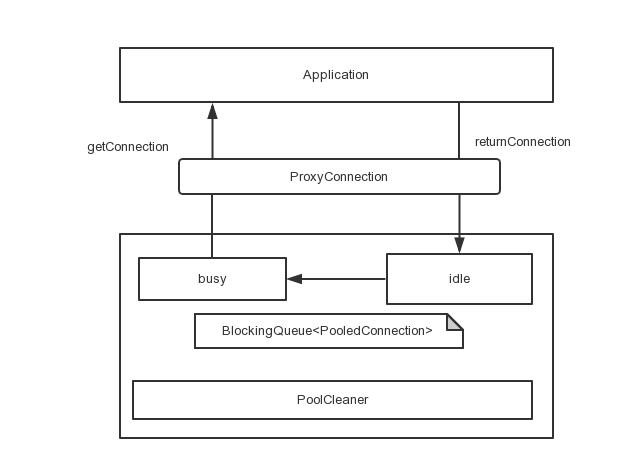
\includegraphics[width=130mm]{flow-struct-db-connect-pool.png}
    \caption{数据库连接池示意图}
    \label{fig:flow-struct-db-connect-pool}
\end{figure}
\subsubsection{关系型数据库MySQL}
JPA(Java Persistence API),即Java持久层API,是Java EE中标准的对象-关系表的映射接口规范,Spring Data JPA在其之上封装了更简单易
用的使用接口。JPA本身仅是一套接口规范,具体实现依赖Hibernate、OpenJPA等框架。本系统中使用Spring Boot默认的Hibernate框架作为JPA的具
体实现。\par
\begin{figure}[H]
    \centering
    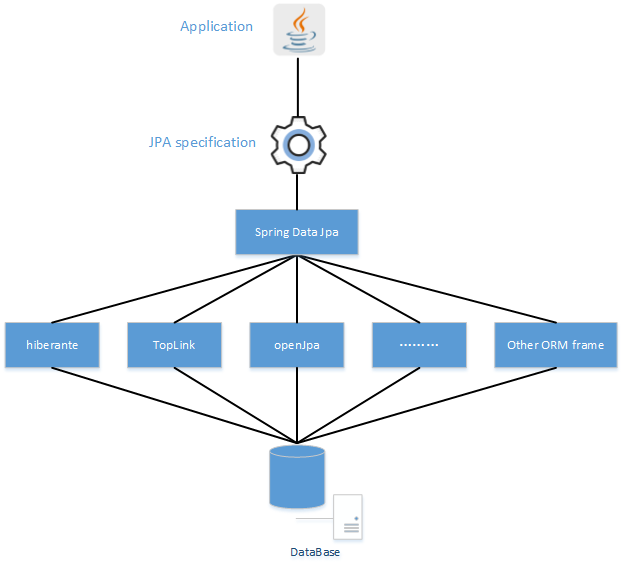
\includegraphics[width=130mm]{struct-jpa.png}
    \caption{JPA规范与具体实现}
    \label{fig:struct-jpa}
\end{figure}
在MySQL数据库规范中,本系统规定了每张表必须包含id、create\_time、creator、modify\_time、modifier、note、version字段。\par
其中create\_time、creator、modify\_time、modifier字段通过定义JPA规范中的审计(audit)功能可以实现在实体对象持久化到数据库中时自动
填充。下面代码是审计(audit)信息提供者的实现,其中获取creator、modifier填充信息时用到了权限拦截器保存到AuthContextHolder中的数据。\par
\begin{mdframed}\begin{verbatim}
@Configuration
@EnableJpaAuditing(auditorAwareRef = "auditorAware", 
                   dateTimeProviderRef = "dateTimeProvider")
@EntityScan(basePackages = ["pc.crs.auth.domain"])
class JpaConfiguration {
    @Bean
    fun auditorAware() = AuditorAware<String> { 
        Optional.of(AuthContextHolder.getUserInfo()?.name ?: "anonymous") 
    }

    @Bean
    fun dateTimeProvider() = CurrentDateTimeProvider.INSTANCE
}
\end{verbatim}\end{mdframed}\par
\begin{mdframed}\begin{verbatim}
@MappedSuperclass
@EntityListeners(AuditingEntityListener::class)
abstract class BaseDO(
        @Id @GeneratedValue(strategy = GenerationType.IDENTITY) 
        var id: Long? = null,
        @CreatedBy @Column(nullable = false) 
        var creator: String = "",
        @LastModifiedBy @Column(nullable = false) 
        var modifier: String = "",
        @CreatedDate @Column(nullable = false) 
        var createTime: LocalDateTime? = null,
        @LastModifiedDate @Column(nullable = false) 
        var modifiedTime: LocalDateTime? = null,
        @Column(nullable = false, columnDefinition = "text") 
        var note: String = "",
        @Version @Column(nullable = false) 
        var version: Long? = null
) : Serializable
\end{verbatim}\end{mdframed}\par
\begin{mdframed}\begin{verbatim}
@Entity
@Table(name = "acl", indexes = [
    Index(name = "priority_index", columnList = "priority")
])
data class AclDO(
        @Column(nullable = false) var name: String = "",
        @Column(nullable = false, columnDefinition = "text") 
        var url: String = "",
        @Column(nullable = false) var anonymous: Boolean = false,
        @Column(nullable = false) var affirmative: Boolean = false,
        @Column(nullable = false) var permissions: String = "",

        @Convert(converter = LongListJsonConverter::class) 
        @Column(nullable = false)
        var roleIds: List<Long> = emptyList(),

        @Column(nullable = false, 
                columnDefinition = "int COMMENT '数值小优先'") 
        var priority: Int = 100
) : BaseDO()
\end{verbatim}\end{mdframed}\par
定义审计(audit)信息提供者后,还需在实体类中的相应字段添加注解才可实现审计信息自动填充功能。\par
Id字段采用MySQL中自增主键的策略,在实体类中的相应字段添加注解并指定主键生成策略即可实现该功能。\par
Version字段用于乐观锁,其原理是在每个表中增加一个单独字段,用于标记每条记录的版本号。在一个数据库事务中,第一次读取数据时将读取该记录的
版本号,在后续的修改中,每次执行SQL之前均要校验该版本号是否与最初读到的一致,若一致,则认为没有冲突,执行SQL,提交事务,并增加版本号;若
不一致,则认为数据被其他线程或程序修改,本次操作失败,事务回滚。在JPA标准中,只需在实体类中的相应字段添加@Version注解即可实现乐观锁功能。\par
在标准的JDBC驱动中,指定了数据库类型与Java类型的映射关系,在本系统中,为方便开发,自定义扩展了类型映射,允许将MySQL表中的varchar类型
映射成Kotlin中的List类型,其中varchar类型中的数据约定以英文逗号分隔。下为该扩展类型映射转换器的实现,在指定该映射关系时,还需在实体类
上加上@Convert注解。\par
\begin{mdframed}\begin{verbatim}
class LongListJsonConverter : AttributeConverter<List<Long>, String> {
    override fun convertToDatabaseColumn(attribute: List<Long>): String {
        return attribute.joinToString(separator = ",") { it.toString() }
    }

    override fun convertToEntityAttribute(dbData: String): List<Long> {
        return dbData.split(',')
                     .filterNot { it.isBlank() }
                     .map { it.trim().toLong() }
    }
}
\end{verbatim}\end{mdframed}\par

\subsubsection{非关系型数据库Redis}
Redis是一个基于内存的高速NoSQL数据库,其本身仅支持键值对的数据存储,并不具备关系型数据库的检索能力。Spring Data Redis框架中,通过在
实体类上增加注解,可以在存入数据时,由框架自动辅助索引数据,存储在Redis中,以用于按照除主键外的索引字段检索数据。\par
同时,由于Redis将所有数据存放在内存中,存储代价是比较高的,通过在实体类上增加注解,合理设置数据的过期时间,释放存储空间,提高数据库的工作
效率。\par
\begin{mdframed}\begin{verbatim}
@RedisHash(value = "crs:auth:token", timeToLive = 30 * 60)
data class TokenDO(@Id val id: String = UUID.randomUUID().toString(),
                   @Indexed val userId: Long) : Serializable
\end{verbatim}\end{mdframed}\par

\subsection{权限控制实现}
在传统的MVC应用中,由Servlet容器(如Tomcat)维持Session,其原理是在客户端浏览器上通过Cookie保持JSESSIONID,在与服务器通信时携带该信息,
Servlet容器通过JSESSIONID区分Session,整个过程由Servlet容器自动管理。\par
RESTful风格是一种无状态的请求操作,本身并没有Session的概念,每次请求携带用于标识身份的token从服务器获取资源,因此需要通过手工实现类似
Session的功能。\par
本系统中,用户登录后服务器将生成一个UUID返回给请求者作为token,并将该token作为键、用户id作为值存入Redis缓存中,设定30分钟的过期时间。请求
者在每次请求是携带该token作为唯一身份标识。\par
\subsubsection{工作流程}
\begin{figure}[H]
    \centering
    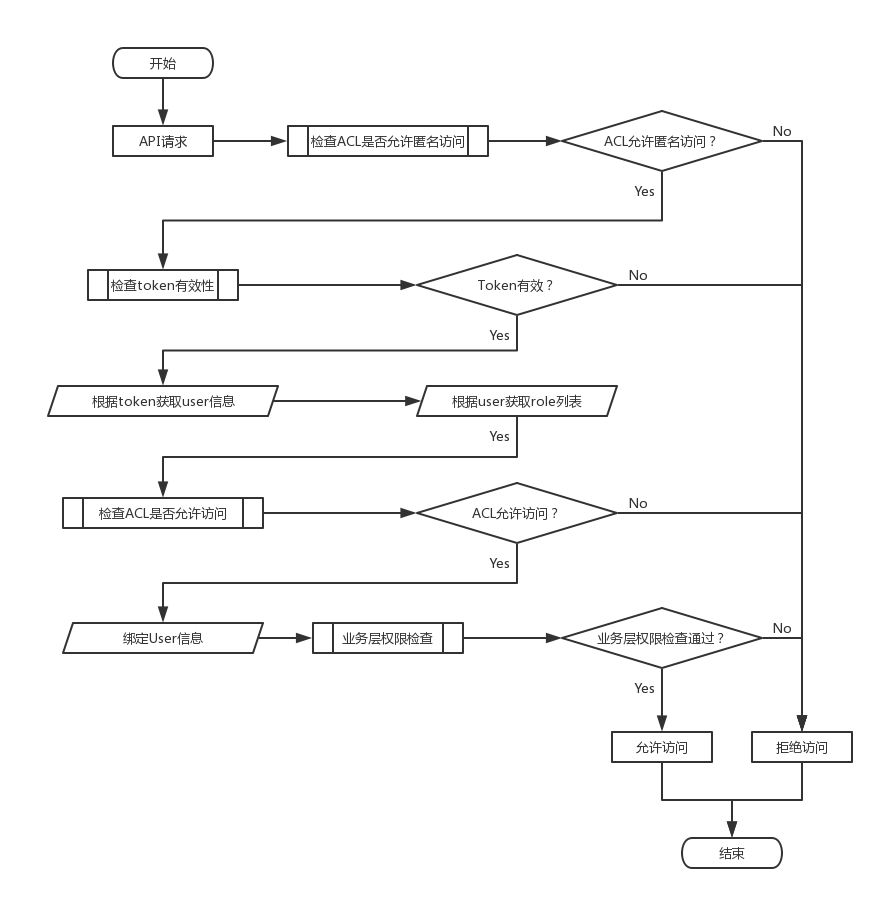
\includegraphics[width=150mm]{flow-auth.png}
    \caption{权限控制流程图}
    \label{fig:flow-auth}
\end{figure}
\subsubsection{请求拦截}
\begin{figure}[H]
    \centering
    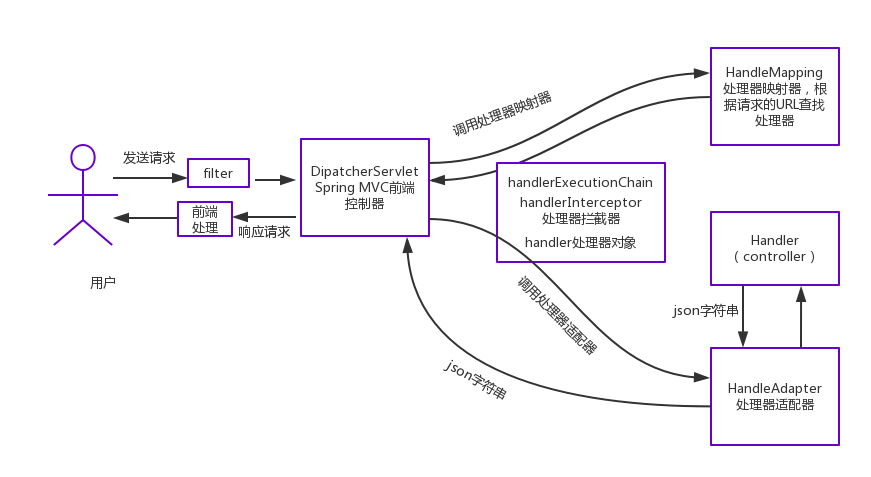
\includegraphics[width=150mm]{flow-spring-mvc-restful.png}
    \caption{Spring MVC框架部分工作流程(RESTful模式)}
    \label{fig:flow-spring-mvc-restful}
\end{figure}
图\ref{fig:flow-spring-mvc-restful}中标识了Spring MVC框架在使用RESTful模式时的部分工作流程,从图中可以看出,在每次请求到达控制器
(Controller之前),需要经过过滤器(Filter)和拦截器(Interceptor),可以在这里实现权限的校验。若权限校验通过,则放行,继续后续流程;
若权限校验不通过,则终止请求,向请求方发送错误消息。\par
其中过滤器(Filter)是Java EE中的标准组件,拦截器(Interceptor)是Spring MVC框架中的组件。在Spring项目中,拦截器(Interceptor)更
加灵活易用,可以使用Spring框架中诸多特性,因此本系统选择在拦截器(Interceptor)中实现权限控制。\par
\subsubsection{信息传递}
在Spring MVC框架中,DispatchServlet作为前端HTTP请求分发器,支持同步和异步两种线程模式。本系统使用默认的同步模式,该模式下,每一个请求
从被DispatchServlet分发到线程池后,会在其中一个线程内同步执行。因此在权限控制拦截器中,若请求通过权限校验,把请求者的信息存储在线程隔离的
“容器”中,可供后续的处理流程使用。\par
ThreadLocal正是线程隔离的存储容器,本系统中,每个微服务维护一个单例ThreadLocal容器,每个请求在通过权限拦截器时将请求者信息放入其中,并在
请求结束后清空该信息,避免对后续请求造成影响。\par
\begin{mdframed}\begin{verbatim}
object AuthContextHolder {
    private val userInfoHolder 
            = NamedInheritableThreadLocal<UserInfo>("UserInfoHolder")
    fun getUserInfo(): UserInfo? = userInfoHolder.get()
    fun setUserInfo(userInfo: UserInfo) = userInfoHolder.set(userInfo)
    fun clean() = userInfoHolder.remove()
}

data class UserInfo(
        var id: Long? = null,
        var name: String = "",
        var loginName: String = "",
        var affirmative: Boolean = false,
        var token: String = "",
        val roles: List<String> = emptyList()
)
\end{verbatim}\end{mdframed}\par

\subsection{统一日志记录}
本系统使用Spring AOP实现了统一的请求日志记录功能。AOP即面向切面编程,可以非侵入式的在指定切面(如指定的方法)统一前后执行部分逻辑。本项
目中定义了@Log注解作为切面,并支持定义日志级别、排除类型等选项,只需将该注解添加到方法上,即可在调用该方法时打印传入参数和返回结果到日志
文件,用于后期的程序分析和错误排查。
\begin{mdframed}\begin{verbatim}
/**
 * 方法级日志切面注解
 * @author pancheng
 */
@Target(METHOD)
@Retention(RUNTIME)
public @interface Log {
    /**
     * 日志等级,支持 "OFF", "ERROR", "WARN", "DEBUG", "INFO", "TRACE"
     */
    String level() default "INFO";
    /**
     * 是否记录参数
     */
    boolean enableArgs() default true;   
    /**
     * 是否记录返回值
     */
    boolean enableRet() default true;
    /**
     * 忽略记录的类型
     */
    Class<?>[] ignoreTypes() default {ServletRequest.class, 
                                      ServletResponse.class};
}
\end{verbatim}\end{mdframed}\par

\subsection{异常处理}
\subsubsection{自定义异常}
在本系统中,结合具体的业务逻辑,自定义了以下4中异常类:
\begin{itemize}
    \item CriterionException - 表示JPA查询条件解析时发生异常。
    \item NoPermissionException - 表示用户无权操作。
    \item RecordNotFoundException - 表示要访问的数据记录不存在。
    \item ValidateException - 表示数据校验不通过。
\end{itemize}\par
上述4种自定义异常均为非受检异常,直接继承RuntimeException。
\subsubsection{数据库事务}
在业务逻辑的执行过程中,有可能一个业务逻辑对应多次数据库的读写操作,若中途发生异常,业务逻辑执行失败,则需要撤销对数据库已进行的操作,需要
用到数据库的事务特性。\par
在Spring框架中,通AOP实现了事务管理器,仅需要在业务逻辑方法上加上@Transactional注解,即可实现自动的事务管理。默认情况下,若该方法执行
过程中抛出非受检异常,则事务回滚,撤销所有对数据库已有的修改操作,否则提交。\par
\subsubsection{全局异常处理器}
在本系统中,对于大多数异常来说,一旦发生,意味着本次操作失败,并没有后备方案可以执行,所要做的就是将错误日志打印,并返回调用者简要的错误原
因。因此,本系统中引入了全局异常处理器,用于统一处理异常,在业务逻辑方法中,如果发生无可修复的异常,无需捕获,自动向外抛出,最后统一交给全
局异常处理器处理,打印错误日志,并返回调用者简要的错误原因。\par
\begin{mdframed}\begin{verbatim}
abstract class BaseExceptionHandler {
    open val logger: Logger = LoggerFactory.getLogger(this.javaClass)

    @ExceptionHandler(RecordNotFoundException::class)
    fun handleRecordNotFoundException(e: RecordNotFoundException)
            : RestResult {
        logger.error("捕获到异常", e)
        return failureRestResult(e.message ?: "记录不存在")
    }
    // ... 省略其他类型异常处理过程
}

// 向Spring MVC注册自定义异常处理器,并设置最高优先级
@Order(1)
@RestControllerAdvice
class GlobalExceptionHandler : BaseExceptionHandler()
\end{verbatim}\end{mdframed}\par

\subsection{文件服务器实现}
\subsubsection{实现方案}
本系统中,课程封面、课程资源附件、在线视频等功能均需要使用文件上传与下载功能,因此,专门搭建了一个文件服务器满足该需求。\par
文件服务器由一个微服务和Nginx服务组成。微服务用于接受和分类文件上传,将文件按一定的规则存储在磁盘上,并将文件信息存储到数据库;
Nginx服务负责文件下载,当请求文件下载时,Nginx服务器根据URL解析文件路径,并向请求方传输文件流。\par
\subsubsection{时序图}
\begin{figure}[H]
    \centering
    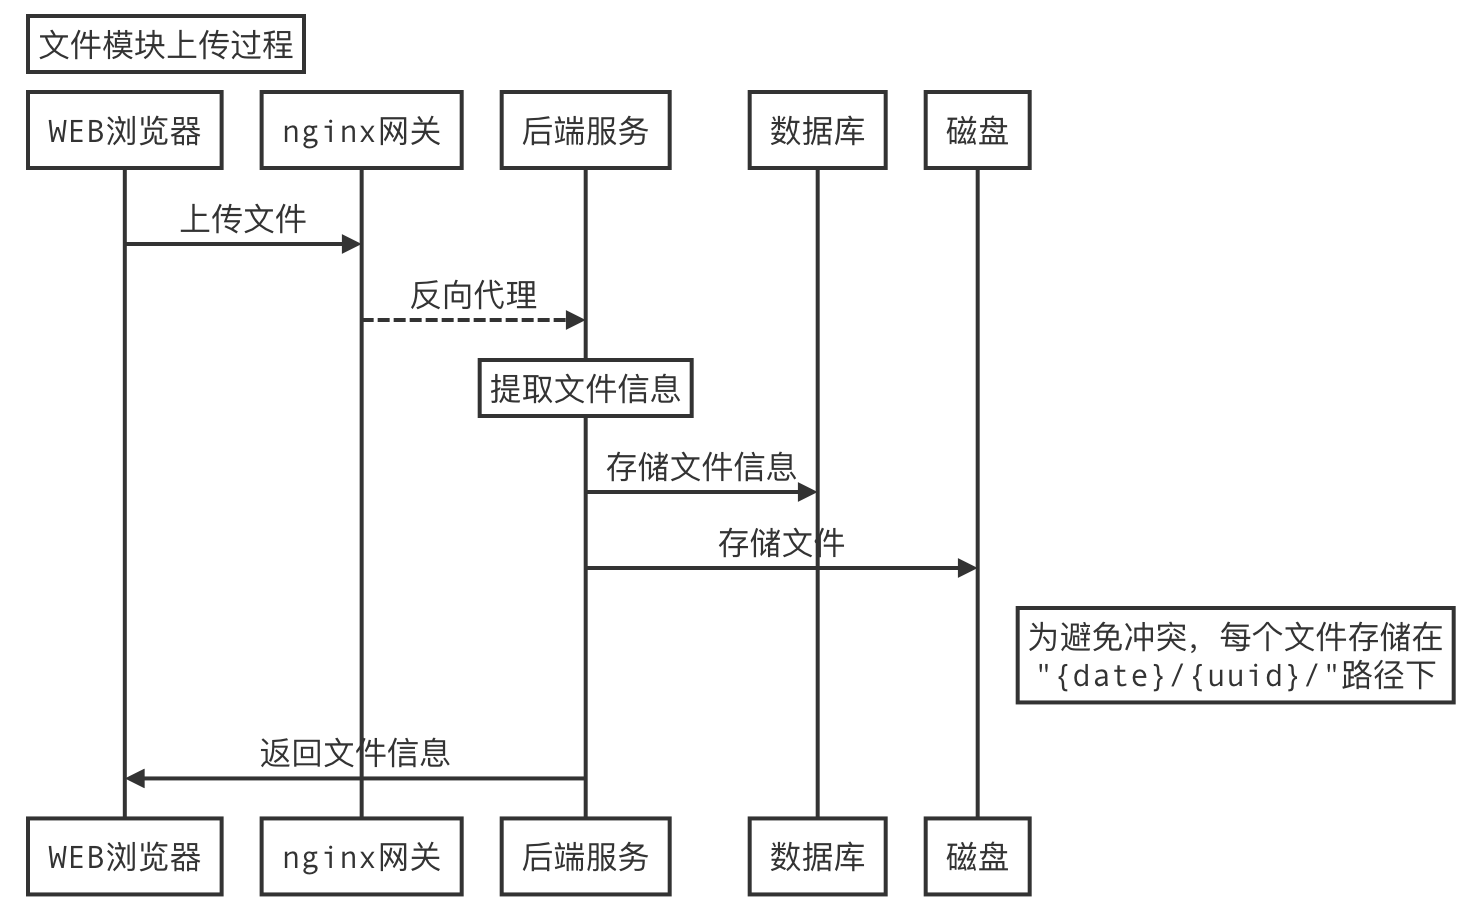
\includegraphics[width=150mm]{seq-file-upload.png}
    \caption{文件模块上传过程时序图}
    \label{fig:seq-file-upload}
\end{figure}
\begin{figure}[H]
    \centering
    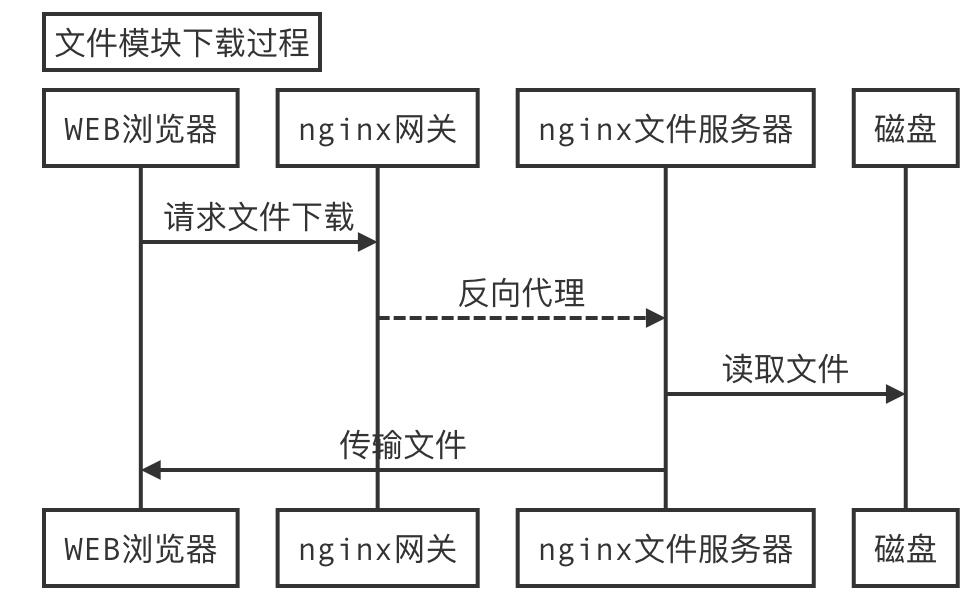
\includegraphics[width=100mm]{seq-file-download.png}
    \caption{文件模块下载过程时序图}
    \label{fig:seq-file-download}
\end{figure}

\subsection{通用查询解析器}
本系统在数据库设计时,不是完全遵守关系数据库设计范式,而是尽可能以业务切分表格和数据库。因此,在系统开发过程中,将会有大量的单表查询需求,为了提高代码的复用率,
设计了一个通用查询解析器,可以实现一键单表查询,并支持排序、分页功能。\par
\subsubsection{属性查询}
\begin{figure}[H]
    \centering
    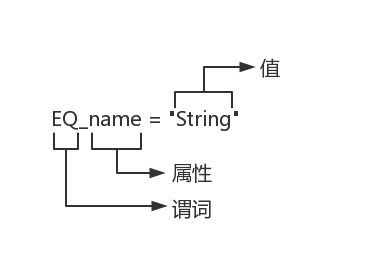
\includegraphics[width=100mm]{query_field.png}
    \caption{属性查询短语}
    \label{fig:query_field}
\end{figure}

\begin{longtable}{|p{10em}|p{6em}|p{15em}|}
	\caption{通用属性查询短语表}\label{tab:query_field}   \\\hline
	谓词 & 语义       & 说明                              \\\hline
	\endfirsthead
	\multicolumn{3}{r}{{续\tablename\thetable{}}}         \\\hline
	\endhead
	EQ   & 相等       & 精确匹配,对应SQL中=              \\\hline
	NEQ  & 不相等     & 精确匹配,对应SQL中!=             \\\hline
	LIKE & 相似       & 模糊匹配,对应SQL中LIKE           \\\hline
	GT   & 大于       & 作用字段必须支持比较,对应SQL中>  \\\hline
	LT   & 小于       & 作用字段必须支持比较,对应SQL中<  \\\hline
	GTE  & 大于或等于 & 作用字段必须支持比较,对应SQL中>= \\\hline
	LTE  & 小于或等于 & 作用字段必须支持比较,对应SQL中<= \\\hline
	IN   & 包含       & 范围匹配,对应SQL中IN             \\\hline
	NIN  & 不包含     & 范围匹配,对应SQL中NOT IN         \\\hline
\end{longtable}\par
\subsubsection{排序查询}
\begin{figure}[H]
    \centering
    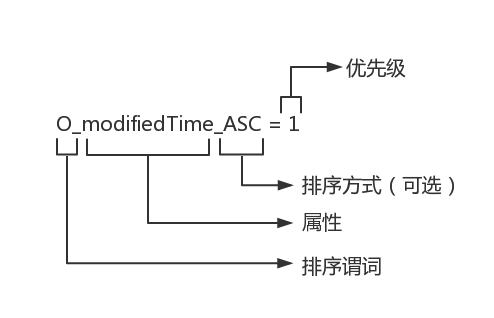
\includegraphics[width=100mm]{query_order.png}
    \caption{属性查询短语}
    \label{fig:query_order}
\end{figure}
排序查询短语由谓词“O”表示,是“order”一词的首字母缩写,短语尾部的排序方式共支持3中,如表\ref{tab:query_order}所示。
\begin{longtable}{|p{10em}|p{6em}|p{15em}|}
	\caption{通用排序查询短语表}\label{tab:query_order} \\\hline
	排序方式 & 语义 & 说明                              \\\hline
	\endfirsthead
	\multicolumn{3}{r}{{续\tablename\thetable{}}}       \\\hline
	\endhead
	缺省     & 默认 & 默认为增序,与SQL默认语义一致     \\\hline
	ASC      & 增序 & 字段按增序排序                    \\\hline
	DESC     & 降序 & 字段按降序排序                    \\\hline
\end{longtable}\par
\subsubsection{分页查询}
\begin{figure}[H]
    \centering
    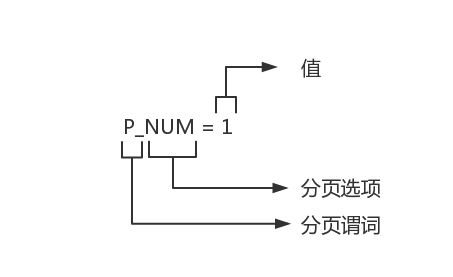
\includegraphics[width=100mm]{query_page.png}
    \caption{属性查询短语}
    \label{fig:query_page}
\end{figure}
分页查询短语由谓词“P”表示,是“page”一词的首字母缩写,用于控制查询结果的分页,以改善大表查询时大量数据传输造成的性能和内存、宽带占用问题,
其选项共支持3种,如表\ref{tab:query_order}所示。
\begin{longtable}{|p{10em}|p{6em}|p{15em}|}
	\caption{通用分页查询短语表}\label{tab:query_page} \\\hline
	选项    & 语义     & 说明                          \\\hline
	\endfirsthead
	\multicolumn{3}{r}{{续\tablename\thetable{}}}      \\\hline
	\endhead
	NUM     & 查询页码 & 从0开始,默认为0              \\\hline
	SIZE    & 每页数量 & 默认为10                      \\\hline
	DISABLE & 分页开关 & 默认开启分页功能              \\\hline
\end{longtable}\par

\subsection{自动化部署与维护}
\subsubsection{发布流程}
\begin{figure}[H]
    \centering
    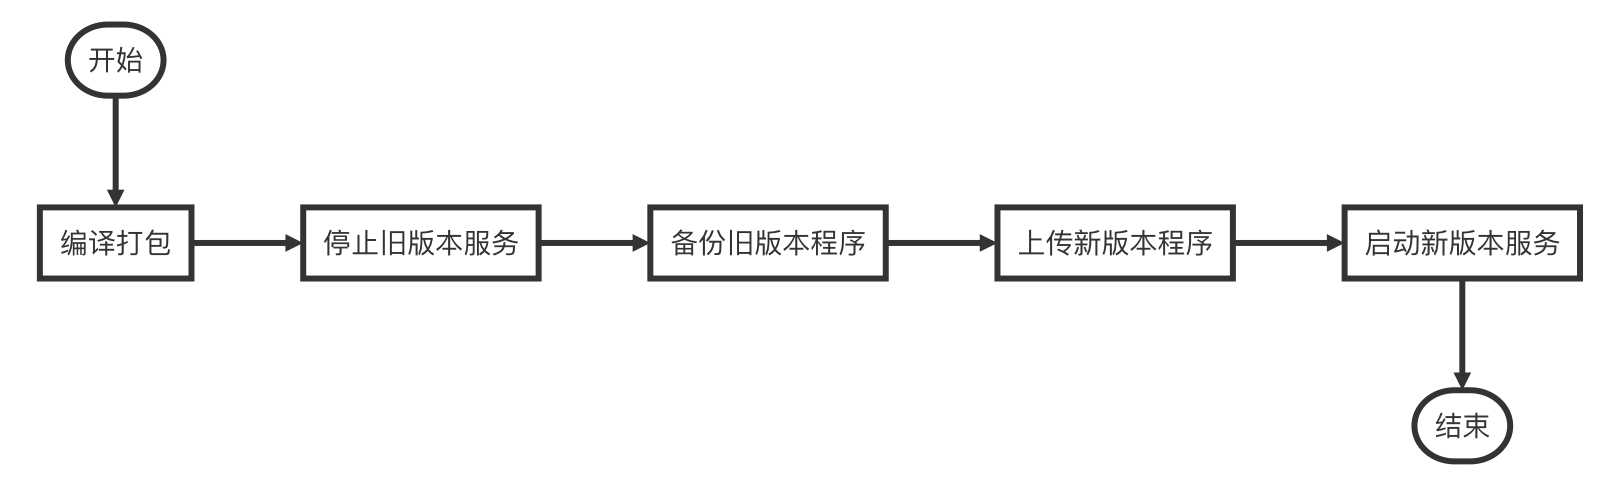
\includegraphics[width=150mm]{flow-deploy.png}
    \caption{微服务升级发布流程}
    \label{fig:flow-deploy}
\end{figure}
\subsubsection{自动化方案}
上述版本发布流程是固定的,因此考虑通过脚本实现自动化。在脚本语言的选择中,发现采用单一的脚本语言实现所有需求难度较大,经考虑,采用多种
脚本加工具链组合的方式,充分发挥各种脚本和工具链特长,协同完成自动化升级部署的任务。\par
\paragraph{编译打包}
使用Gradle自动化打包工具,通过gradle spring-boot插件中的task bootJar将微服务打包。特别的,通过配置插件属性,可以实现将服务打包
成可在Unix-like平台下完全自启动(full executable)的程序包。\par
\paragraph{服务的启动和停止}
本系统将每个微服务作为Linux系统中的守护进程运行,使用Linux系统组件中的systemd管理项目的启动和停止。自定义systemd启动脚本如下:
\begin{mdframed}\begin{verbatim}
[Unit]
Description=crs-file-server
After=syslog.target

[Service]
User=root
ExecStart=/root/crs-bin/crs-file-server.jar
SuccessExitStatus=143

[Install]
WantedBy=multi-user.target
\end{verbatim}\end{mdframed}\par
将上述脚本命名为crs-file-server.service,赋予777权限,放置到/etc/systemd/system目录下,并在crs-file-server.jar同级目下建立
配置文件,命名为crs-file-server.conf,指定启动配置如下:
\begin{mdframed}\begin{verbatim}
JAVA_OPTS='-Xmx512M'
RUN_ARGS='--spring.profiles.active=online \
          --eureka.instance.prefer-ip-address=true \
          --eureka.instance.ip-address=101.132.159.21'
\end{verbatim}\end{mdframed}\par
配置完成后,即可以通过systemctl start crs-file-server.service命令启动该服务,通过systemctl stop crs-file-server.service
命令停止该服务。\par
\paragraph{备份旧版本程序}
直接使用Linux中mv命令,将旧版本程序重命名为以日期时间结尾的名称,即可完成备份。
\paragraph{上传新版本程序}
使用gradle的ssh插件,并配置生成一对rsa公钥和私钥文件,将公钥填写到服务的白名单中,配置ssh插件通过rsa认证方式连接服务器,并执行文件
上传动作。Gradle脚本如下:
\begin{mdframed}\begin{verbatim}
remotes {
    aliyunServer {
        host = '47.100.96.14'
        user = 'root'
        identity = file("${rootDir}/id_rsa")
    }
}
static def now() {
    new Date().format('yyyy-MM-dd-HH:mm:ss')
}
task deploy(dependsOn: pkg) << {
    ssh.run {
        session(remotes.aliyunServer) {
            execute 'systemctl stop crs-server.service'
            execute "mv /root/crs-bin/crs-server.jar" 
                    + "/root/crs-bin/crs-server-${now()}.jar", 
                    ignoreError: true
            put from: "${buildDir}/libs/crs-server-0.0.1-SNAPSHOT.jar", 
                into: '/root/crs-bin/crs-server.jar'
            execute 'chmod u+x /root/crs-bin/crs-server.jar'
            execute 'systemctl start crs-server.service'
        }
    }
}
\end{verbatim}\end{mdframed}\par
\paragraph{脚本协作}
上述的Gradle脚本中,通过execute函数执行Linux命令,以完成服务备份、启动、停止的功能,达到脚本协作的目的,并将该动作定义为一个task,即
可在项目根目录执行gradle deploy实现项目的一键升级发布,达到自动化部署的目的。

\clearpage

\section{测试}
\subsection{测试版本}
\begin{itemize}
    \item 测试地址:\url{http://101.132.159.21/crs/}
    \item 测试账号:admin/admin
\end{itemize}

\subsection{测试内容}
\begin{longtable}{|p{8em}|p{4em}|p{25em}|}
    \caption{测试内容表}\label{tab:test_content} \\\hline
    测试名称         & 测试人员 & 测试内容 \\\hline
    \endfirsthead
    \multicolumn{3}{r}{{续\tablename\thetable{}}} \\\hline
    \endhead
    权限系统测试     & 潘成     & 登录、用户管理、角色管理、访问控制列表管理 \\\hline
    课程资源系统测试 & 潘成     & 课程分类管理、导航栏课程分类列表展示、课程资源增删改查、卡片功能编辑、卡片附件上传、课程资源内容展示、首页热门课程资源展示 \\\hline
    在线测试系统测试 & 潘成     & 题库管理、题目答案编辑、试卷管理、试卷试题组装、试卷展示 \\\hline
    论坛系统测试     & 潘成     & 板块管理、发帖、回帖、删帖 \\\hline
\end{longtable}

\subsection{测试用例}
\subsubsection{权限系统模块}
\begin{longtable}{|p{4em}|p{14em}|p{7em}|p{7em}|p{2em}|}
    \caption{测试内容表}\label{tab:test_auth}  \\\hline
    用例编号    & 用例描述 & 预期结果 & 实际结果 & 备注 \\\hline
    \endfirsthead
    \multicolumn{5}{r}{{续\tablename\thetable{}}}       \\\hline
    \endhead
    权限系统001 &
    前置条件:数据库用户表中已经正确录入用户信息,从其他界面跳转到登录界面。步骤:1.在登录名输入框中输入admin;2.在密码输入框中输入admin;3.点击登录按钮。 &
    登录成功,跳转到登录前的界面,顶栏右侧显示用户名和注销按钮。 &
    登录成功,跳转到登录前的界面,顶栏右侧显示用户名和注销按钮。 &
    通过 \\\hline
    权限系统002 &
    前置条件:用户已登录。步骤:1.点击顶栏注销按钮。 &
    注销成功,顶栏右侧显示登录按钮。 &
    注销成功,顶栏右侧显示登录按钮。 &
    通过 \\\hline
    权限系统003 &
    前置条件:用户在上一次登录成功时勾选了记住密码功能。步骤:1.点击顶栏登录按钮。 &
    跳转到登录界面,并自动填充上次的登录名和密码。 &
    跳转到登录界面,并自动填充上次的登录名和密码。 &
    通过 \\\hline
    权限系统004 &
    前置条件:用户在上一次登录成功时勾选了记住密码和自动登录功能。步骤:1.点击顶栏登录按钮。 &
    直接通过上次登录的用户登录系统。 &
    直接通过上次登录的用户登录系统。 &
    通过 \\\hline
    权限系统005 &
    前置条件:用户已登录,并有相关操作权限;进入到用户管理界面。步骤:1.点击添加按钮,输入相关信息,确定;2.点击列表记录的删除按钮,确定;3.点击列表记录的修改按钮,修改相关信息,确定;4.填写检索条件,点击检索。 &
    系统能正确响应对用户的增删改查操作,及时刷新的展示列表上。 &
    系统能正确响应对用户的增删改查操作,及时刷新的展示列表上。 &
    通过 \\\hline
    权限系统006 &
    前置条件:用户已登录,并有相关操作权限;进入到用户管理界面。步骤:1.点击列表记录的修改按钮,输入新密码,确定。 &
    修改密码成功,该用户可以用新密码登录系统。 &
    修改密码成功,该用户可以用新密码登录系统。 &
    通过 \\\hline
    权限系统007 &
    前置条件:用户已登录,并有相关操作权限;进入到角色管理界面。步骤:1.点击添加按钮,输入相关信息,确定;2.点击列表记录的删除按钮,确定;3.点击列表记录的修改按钮,修改相关信息,确定;4.填写检索条件,点击检索。 &
    系统能正确响应对角色的增删改查操作,及时刷新的展示列表上;用户管理、访问控制列表管理界面上的角色候选框中能够正确显示当前角色列表。 &
    系统能正确响应对角色的增删改查操作,及时刷新的展示列表上;用户管理、访问控制列表管理界面上的角色候选框中能够正确显示当前角色列表。 &
    通过 \\\hline
    权限系统008 &
    前置条件:用户已登录,并有相关操作权限;进入到访问控制列表管理界面。步骤:1.点击添加按钮,输入相关信息,确定;2.点击列表记录的删除按钮,确定;3.点击列表记录的修改按钮,修改相关信息,确定;4.填写检索条件,点击检索。 &
    系统能正确响应对访问控制列表的增删改查操作,及时刷新的展示列表上;访问控制列表能根据优先级自动排序;访问控制列表能正确对绑定角色作用。 &
    系统能正确响应对访问控制列表的增删改查操作,及时刷新的展示列表上;访问控制列表能根据优先级自动排序;访问控制列表能正确对绑定角色作用。 &
    通过 \\\hline
\end{longtable}

\subsubsection{课程资源系统模块}
\begin{longtable}{|p{4em}|p{14em}|p{7em}|p{7em}|p{2em}|}
    \caption{测试内容表}\label{tab:test_course}  \\\hline
    用例编号    & 用例描述 & 预期结果 & 实际结果 & 备注 \\\hline
    \endfirsthead
    \multicolumn{5}{r}{{续\tablename\thetable{}}}       \\\hline
    \endhead
    课程资源系统001 &
    前置条件:用户已登录,并有相关操作权限;进入到分类管理界面。步骤:1.点击添加按钮,输入相关信息,确定;2.点击列表记录的删除按钮,确定;3.点击列表记录的修改按钮,修改相关信息,确定;4.填写检索条件,点击检索。 &
    系统能正确响应对课程分类的增删改查操作,及时刷新的展示列表上;主页导航栏菜单上正确显示所有课程分类;主页可以显示有课程的分类板块。 &
    系统能正确响应对课程分类的增删改查操作,及时刷新的展示列表上;主页导航栏菜单上正确显示所有课程分类;主页可以显示有课程的分类板块。 &
    通过 \\\hline
    课程资源系统002 &
    前置条件:用户已登录,并有相关操作权限;进入到课程管理界面。步骤:1.点击添加按钮,输入相关信息,确定;2.点击列表记录的删除按钮,确定;3.点击列表记录的修改按钮,修改相关信息,确定;4.填写检索条件,点击检索。 &
    系统能正确响应对课程的增删改查操作,及时刷新的展示列表上;在主页热门课程上正确显示;在课程列表页、课程详情页上正确展示。 &
    系统能正确响应对课程的增删改查操作,及时刷新的展示列表上;在主页热门课程上正确显示;在课程列表页、课程详情页上正确展示。 &
    通过 \\\hline
    课程资源系统003 &
    前置条件:用户已登录,并有相关操作权限;进入到课程管理界面。步骤:1.点击列表记录图片列上传按钮;2.拖动图片到上传框或者点击上传框选择图片。 &
    课程封面设定成功,展示列表上的上传按钮变成预览按钮;可以在展示列表上预览封面;课程封面正确展示到主页、课程列表页、课程详情页上。 &
    课程封面设定成功,展示列表上的上传按钮变成预览按钮;可以在展示列表上预览封面;课程封面正确展示到主页、课程列表页、课程详情页上。 &
    通过 \\\hline
    课程资源系统004 &
    前置条件:用户已登录,并有相关操作权限;进入到课程管理界面;已有设定封面的课程。步骤:1.点击列表记录图片列预览按钮;2.点击删除,并确定。 &
    课程封面删除成功,展示列表上的预览按钮变成上传按钮;主页、课程列表页、课程详情页上,该课程显示默认图片上。&
    课程封面删除成功,展示列表上的预览按钮变成上传按钮;主页、课程列表页、课程详情页上,该课程显示默认图片上。&
    通过 \\\hline
    课程资源系统005 &
    前置条件:用户已登录,并有相关操作权限;进入到课程管理界面。步骤:1.点击列表记录卡片列新增卡片按钮;2.输入卡片标题、卡片内容,上传附件,点击确定按钮。 &
    课程卡片添加成功,展示列表上卡片列显示该卡片标题;课程详情页正确展示卡片内容,附件自动分类,PDF可以在线预览,视频可以在线播放,其他附件可直接下载。&
    课程卡片添加成功,展示列表上卡片列显示该卡片标题;课程详情页正确展示卡片内容,附件自动分类,PDF可以在线预览,视频可以在线播放,其他附件可直接下载。&
    通过 \\\hline
    课程资源系统006 &
    前置条件:用户已登录,并有相关操作权限;进入到课程管理界面;已有添加卡片的课程。步骤:1.点击列表卡片列其中一个卡片按钮;2.点击删除,并确定。 &
    点击卡片按钮后显示卡片内容;删除卡片后,展示列表上该卡片按钮消失;课程详情页该卡片内容不再显示。&
    点击卡片按钮后显示卡片内容;删除卡片后,展示列表上该卡片按钮消失;课程详情页该卡片内容不再显示。&
    通过 \\\hline

\end{longtable}

\subsubsection{在线测试系统模块}
\begin{longtable}{|p{4em}|p{14em}|p{7em}|p{7em}|p{2em}|}
    \caption{测试内容表}\label{tab:test_exam}  \\\hline
    用例编号    & 用例描述 & 预期结果 & 实际结果 & 备注 \\\hline
    \endfirsthead
    \multicolumn{5}{r}{{续\tablename\thetable{}}}       \\\hline
    \endhead
    在线测试系统001 &
    前置条件:用户已登录,并有相关操作权限;进入到题库管理界面。步骤:1.点击添加按钮,输入相关信息,确定;2.点击列表记录的删除按钮,确定;3.点击列表记录的修改按钮,修改相关信息,确定;4.填写检索条件,点击检索。 &
    系统能正确响应对问题的增删改查操作,及时刷新的展示列表上。 &
    系统能正确响应对问题的增删改查操作,及时刷新的展示列表上。 &
    通过 \\\hline
    在线测试系统002 &
    前置条件:用户已登录,并有相关操作权限;进入到题库管理界面。步骤:1.点击列表题目/答案列新增按钮;2.填写题目、答案内容,确定。 &
    展示列表上新增按钮变为编辑按钮,点击后可以展示题目、答案内容。 &
    展示列表上新增按钮变为编辑按钮,点击后可以展示题目、答案内容。 &
    通过 \\\hline
    在线测试系统003 &
    前置条件:用户已登录,并有相关操作权限;进入到考试管理界面。步骤:1.点击添加按钮,输入相关信息,确定;2.点击列表记录的删除按钮,确定;3.点击列表记录的修改按钮,修改相关信息,确定;4.填写检索条件,点击检索。 &
    系统能正确响应对问题的增删改查操作,及时刷新的展示列表上;在线考试页能正确展示考试列表。 &
    系统能正确响应对问题的增删改查操作,及时刷新的展示列表上;在线考试页能正确展示考试列表。 &
    通过 \\\hline
    在线测试系统004 &
    前置条件:用户已登录,并有相关操作权限;进入到考试管理界面。步骤:1.点击列表题目列编辑按钮;2.从穿梭框中选择考试题目,点击确定按钮。 &
    展示列表上预览按钮可以正确显示该考试设定的题目和答案;在线考试详情页上能正确展示该考试的题目和答案,答案默认折叠,点击后显示。 &
    展示列表上预览按钮可以正确显示该考试设定的题目和答案;在线考试详情页上能正确展示该考试的题目和答案,答案默认折叠,点击后显示。 &
    通过 \\\hline

\end{longtable}

\subsubsection{论坛系统模块}
\begin{longtable}{|p{4em}|p{14em}|p{7em}|p{7em}|p{2em}|}
    \caption{测试内容表}\label{tab:test_forum}  \\\hline
    用例编号    & 用例描述 & 预期结果 & 实际结果 & 备注 \\\hline
    \endfirsthead
    \multicolumn{5}{r}{{续\tablename\thetable{}}}       \\\hline
    \endhead
    论坛系统001 &
    前置条件:用户已登录,并有相关操作权限;进入到论坛版块管理界面。步骤:1.点击添加按钮,输入相关信息,确定;2.点击列表记录的删除按钮,确定;3.点击列表记录的修改按钮,修改相关信息,确定;4.填写检索条件,点击检索。 &
    系统能正确响应对论坛版块的增删改查操作,及时刷新的展示列表上;论坛页上能正确展示版块标签。 &
    系统能正确响应对论坛版块的增删改查操作,及时刷新的展示列表上;论坛页上能正确展示版块标签。 &
    通过 \\\hline
    论坛系统002 &
    前置条件:用户已登录,并有相关操作权限;进入到论坛界面。步骤:1.点击发帖按钮;2.填写帖子内容,点击确定按钮。 &
    论坛界面能正确展示板块标签、帖子列表、帖子热度、最新回复时间等信息;发帖后帖子能够正确显示在列表。 &
    论坛界面能正确展示板块标签、帖子列表、帖子热度、最新回复时间等信息;发帖后帖子能够正确显示在列表。 &
    通过 \\\hline
    论坛系统003 &
    前置条件:用户已登录,并有相关操作权限;进入到帖子详情页。步骤:1.点击回帖按钮;2.输入回帖内容,点击确定按钮。 &
    帖子详情页能正确展示帖子内容以及每条回帖内容,回帖自动编楼;回帖后,回帖内容能够正确显示。 &
    帖子详情页能正确展示帖子内容以及每条回帖内容,回帖自动编楼;回帖后,回帖内容能够正确显示。 &
    通过 \\\hline
    论坛系统004 &
    前置条件:用户已登录,并有相关操作权限;进入到帖子管理界面;数据库中已存入帖子数据。步骤:1.填写检索条件,点击检索;2.点击列表记录的删除按钮,确定。 &
    系统能正确响应对帖子的检索和删除操作,及时刷新的展示列表上。 &
    系统能正确响应对帖子的检索和删除操作,及时刷新的展示列表上。 &
    通过 \\\hline

\end{longtable}

\clearpage

\section{小结}
至此,我的毕业设计将告一段落。从2017年11月题目确定以来,整个毕业设计已持续了半年有余,在此期间所做的努力,终有一定的成果,并学到了大量的新知识,对个人能力有莫大的提高。\par
本设计的主要意义即是对软件工程新框架、新技术、新思维的探索与尝试。在系统设计过程中,决定大胆采用软件工程新技术,包括全新的Kotlin语言、Spring Cloud分布式微服务框架、Vue框架、
Gradle构建工具等。在使用新技术时,一方面通传统技术进行比较,打破思维的局限,深入理解其全新的设计思想的优势;另一方面,面对新技术资料的匮乏,不得不进行更多的自我尝试、仔细专研
官方文档,甚至深入源码调试、与开发者讨论。整个过程,我的技术视野不断扩宽,技术能力有了极大的提高。\par
在撰写本论文之前,我对软件工程不曾有系统的学习,不熟悉传统软件工程中瀑布流的开发模式与文档撰写,通过请教学长、参考书籍文献资料对这部分知识进行了补充,是本次论文的一大收获。\par
技术的发展,是一个不断前进与革新的过程,不仅仅是对现有技术的改善,更有对传统技术的摒弃和全新技术的大胆探索,面对日新月异的技术,既要要不断的学习,更要不停的思考,透过表象看清
技术的本质和思想,适时摒弃过时的思想,拥抱新的思维,做好技术沉淀与创新。\par
我的学生时代即将结束,四年的大学生活过的非常充实,学业、思想、能力都得到了充分的培养和锻炼,现在我即将步入社会,这是一个新的开始,我对未来充满着信心,在工作路上,我会不忘初心,
砥砺前进。\par
\clearpage

\section*{谢辞}
本毕业设计是在周平老师的指导下完成的。首先要感谢周平老师包容的态度以及严谨的治学态度。在确定系统开发技术时,周老师允许我采用较新的技术;在后续的汇报交流过程中,周老师针对我的系统
设计提出了很多宝贵的修改意见,并严格督促毕业设计进度。\par
我要感谢实习公司的领导和同事。一方面感谢领导在实习期间尽量少给我安排工作任务,并允许我在实习空余时间进行毕业设计;另一方面感谢许多同事在技术方面给我很多帮助,每次请教他们技术问题
都会得到热情的回复和耐心的讲解。\par
我要感谢全世界的开发者,感谢他们对这个行业所做的贡献,感谢他们的奉献精神,他们开发并开源了如此众多的优秀技术框架无偿供我们学习和使用,正是他们,驱动着整个信息技术产业的发展和进步。\par
感谢学生时代陪我一路走过的同学、朋友们以及我的家人,学生时代,离不开这些和我最近的人。\par
\clearpage

\begin{thebibliography}{99}
    \bibitem{kotlin} Kotlin官方网站,\url{http://kotlinlang.org/}
    \bibitem{spring-cloud} Spring Cloud官方网站,\url{http://projects.spring.io/spring-cloud/}
    \bibitem{gradle} Gradle官方网站,\url{https://gradle.org/}
    \bibitem{vue} Vue.js官方网站,\url{https://cn.vuejs.org/}
    \bibitem{webpack} Webpack官方网站,\url{http://webpack.github.io/}
    \bibitem{2017政府工作报告} 2017年政府工作报告,\url{http://www.gov.cn/premier/2017-03/16/content_5177940.htm}
    \bibitem{第40次中国互联网络发展状况统计报告} 第40次中国互联网络发展状况统计报告,中央网络安全和信息化领导小组办公室、国家互联网信息办公室、中国信息网络互联中心,2017年8月
    \bibitem{jetbrains} Jetbrains官方网站,\url{http://www.jetbrains.com/}
\end{thebibliography}
\end{document}
